%%%%%%%%%%%%%%%%%%%%%%%%%%%%%%%%%%%%%%%%%%%%%%%%%%%%%%%%%%%%%%%%%%%%%%%%%%%
%  TP2 - Parte 1: Modelado de transmisores ópticos con MZM
%  Ejercicios 1 a 4
%  Figuras generadas con los testbench del repo Repo_Com2_Fulgor:
%    Ej. 1   -> tests/testbench_Laser.m
%    Ej. 2-3 -> tests/testbench_MZM.m
%    Ej. 4   -> tests/test_MZM_ex4.m
%%%%%%%%%%%%%%%%%%%%%%%%%%%%%%%%%%%%%%%%%%%%%%%%%%%%%%%%%%%%%%%%%%%%%%%%%%%

\section*{PARTE 1: Modelado de transmisores ópticos con MZM}

La simulación trabaja con el campo eléctrico en banda base compleja
equivalente, normalizado de modo que $|E(t)|^2$ es la potencia óptica
instantánea en [W]; por lo tanto el campo se expresa en $[\sqrt{\text{W}}]$.
Salvo que se indique lo contrario, la frecuencia de muestreo es
$f_s = 960$~GHz.

%==========================================================================
\subsection*{Ejercicio 1: Modelo de un láser}
%==========================================================================

\subsubsection*{Implementación}

El láser de onda continua con ruido se modela como
%
\begin{equation}
E(t) = \sqrt{P_0 + I_n(t)}\;\exp\!\big[\,j\,(2\pi\,FO\,t + \phi_n(t))\big],
\label{eq:ej1_laser}
\end{equation}
%
donde $P_0$ es la potencia media, $I_n(t)$ el ruido de intensidad relativa
(RIN), $FO$ el offset de frecuencia respecto de la portadora nominal y
$\phi_n(t)$ el ruido de fase.

\paragraph{Ruido de intensidad.}
El RIN se define como la densidad espectral unilateral de las fluctuaciones
de potencia normalizada a $P_0^2$. Si $I_n[k]$ es ruido blanco gaussiano
de varianza $\sigma_{RIN}^2$, su densidad unilateral es $2\sigma_{RIN}^2/f_s$,
de donde
%
\begin{equation}
\sigma_{RIN} = P_0\,\sqrt{\frac{RIN\cdot f_s}{2}}.
\label{eq:ej1_rin}
\end{equation}

\paragraph{Ruido de fase.}
Se modela como un proceso de Wiener discreto,
%
\begin{equation}
\phi_n[k] = \phi_n[k-1] + \Delta\phi[k], \qquad
\Delta\phi[k] \sim \mathcal{N}\!\left(0,\ \sigma_\phi^2\right), \qquad
\sigma_\phi^2 = \frac{2\pi\,\Delta\nu}{f_s},
\label{eq:ej1_wiener}
\end{equation}
%
con $\Delta\nu$ el ancho de línea (LW). Un campo con este ruido de fase
tiene una densidad espectral lorentziana (Cauchy--Lorentz) de ancho a media
altura $\Delta\nu$:
%
\begin{equation}
S_E(f) = \frac{P_0}{\pi\,(\Delta\nu/2)}\;
\frac{1}{1 + \left(\dfrac{f-FO}{\Delta\nu/2}\right)^{2}}.
\label{eq:ej1_lorentz}
\end{equation}

\subsubsection*{Verificación}

Cada parámetro se verificó por separado, apagando los ruidos que no
intervienen en la medición ($RIN = -400$~dB/Hz o $\Delta\nu = 0$). Se
barrieron los valores pedidos por la consigna:
$P_0 = (10:2:24)$~dBm, $RIN = -(145, 150, 155)$~dB/Hz,
$FO = (-4:4:4)$~GHz y $\Delta\nu = (100:200:1200)$~kHz.

\paragraph{Potencia.}
La potencia estimada como $\langle|E|^2\rangle$ coincide con la configurada
en todo el barrido. El modelo no introduce atenuación sobre $P_0$
(Figura~\ref{fig:ej1_potencia}).

\begin{figure}[H]
\centering
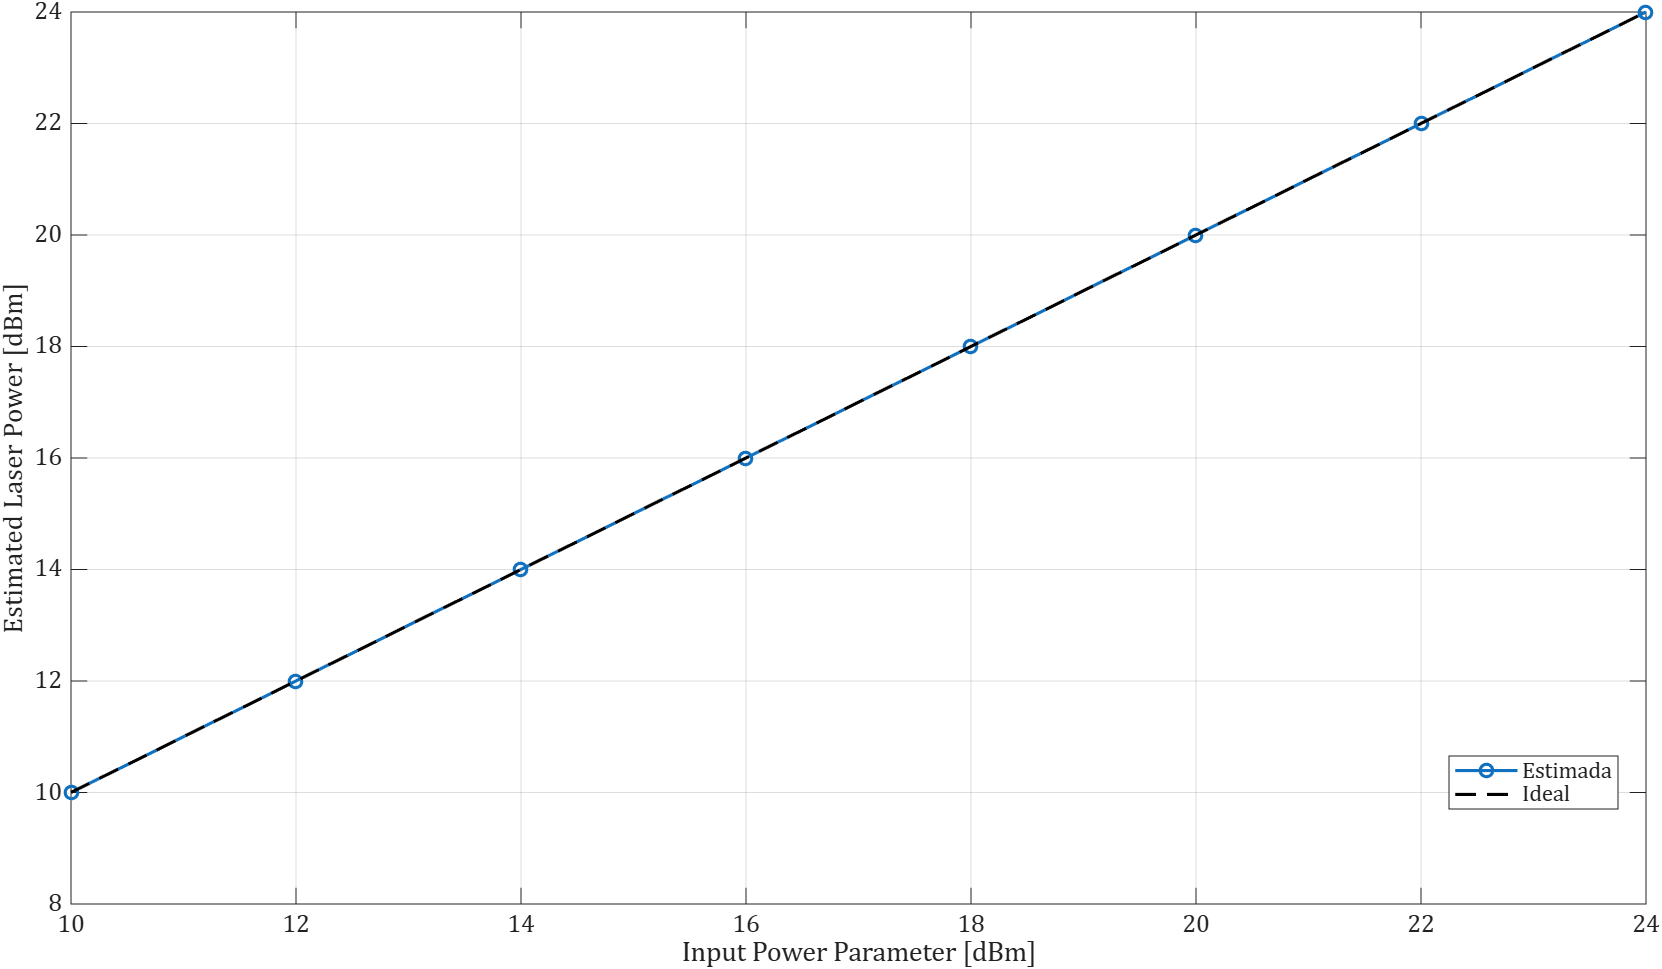
\includegraphics[width=0.7\textwidth]{figuras/ej1_potencia.png}
\caption{Potencia estimada en función de la potencia configurada.}
\label{fig:ej1_potencia}
\end{figure}

\paragraph{Estimación espectral.}
Las densidades espectrales se estimaron con el método de Welch (ventana de
Hann, 50~\% de solapamiento). Una estimación espectral de un proceso
aleatorio es a su vez aleatoria: promediar $K$ segmentos reduce su
dispersión relativa a $\sim 1/\sqrt{K}$, mientras que la resolución la fija
el largo de la ventana. Para suavizar las curvas sin perder resolución se
promediaron además $16$ realizaciones independientes del láser.

\paragraph{RIN.}
Se estimó la densidad espectral de las fluctuaciones de potencia
$|E|^2 - \langle|E|^2\rangle$ y se despejó el RIN invirtiendo la
ecuación~(\ref{eq:ej1_rin}). La densidad es plana en todo el rango de
frecuencias (Figura~\ref{fig:ej1_rin}), lo que confirma que el ruido de
intensidad es blanco, y los valores estimados reproducen los configurados
con error menor a $0.005$~dB (Tabla~\ref{tab:ej1_rin}).

\begin{table}[H]
\centering
\small
\begin{tabular}{cc}
\toprule
RIN configurado [dB/Hz] & RIN estimado [dB/Hz] \\
\midrule
$-145$ & $-145.004$ \\
$-150$ & $-150.002$ \\
$-155$ & $-154.999$ \\
\bottomrule
\end{tabular}
\caption{RIN configurado y estimado.}
\label{tab:ej1_rin}
\end{table}

\begin{figure}[H]
\centering
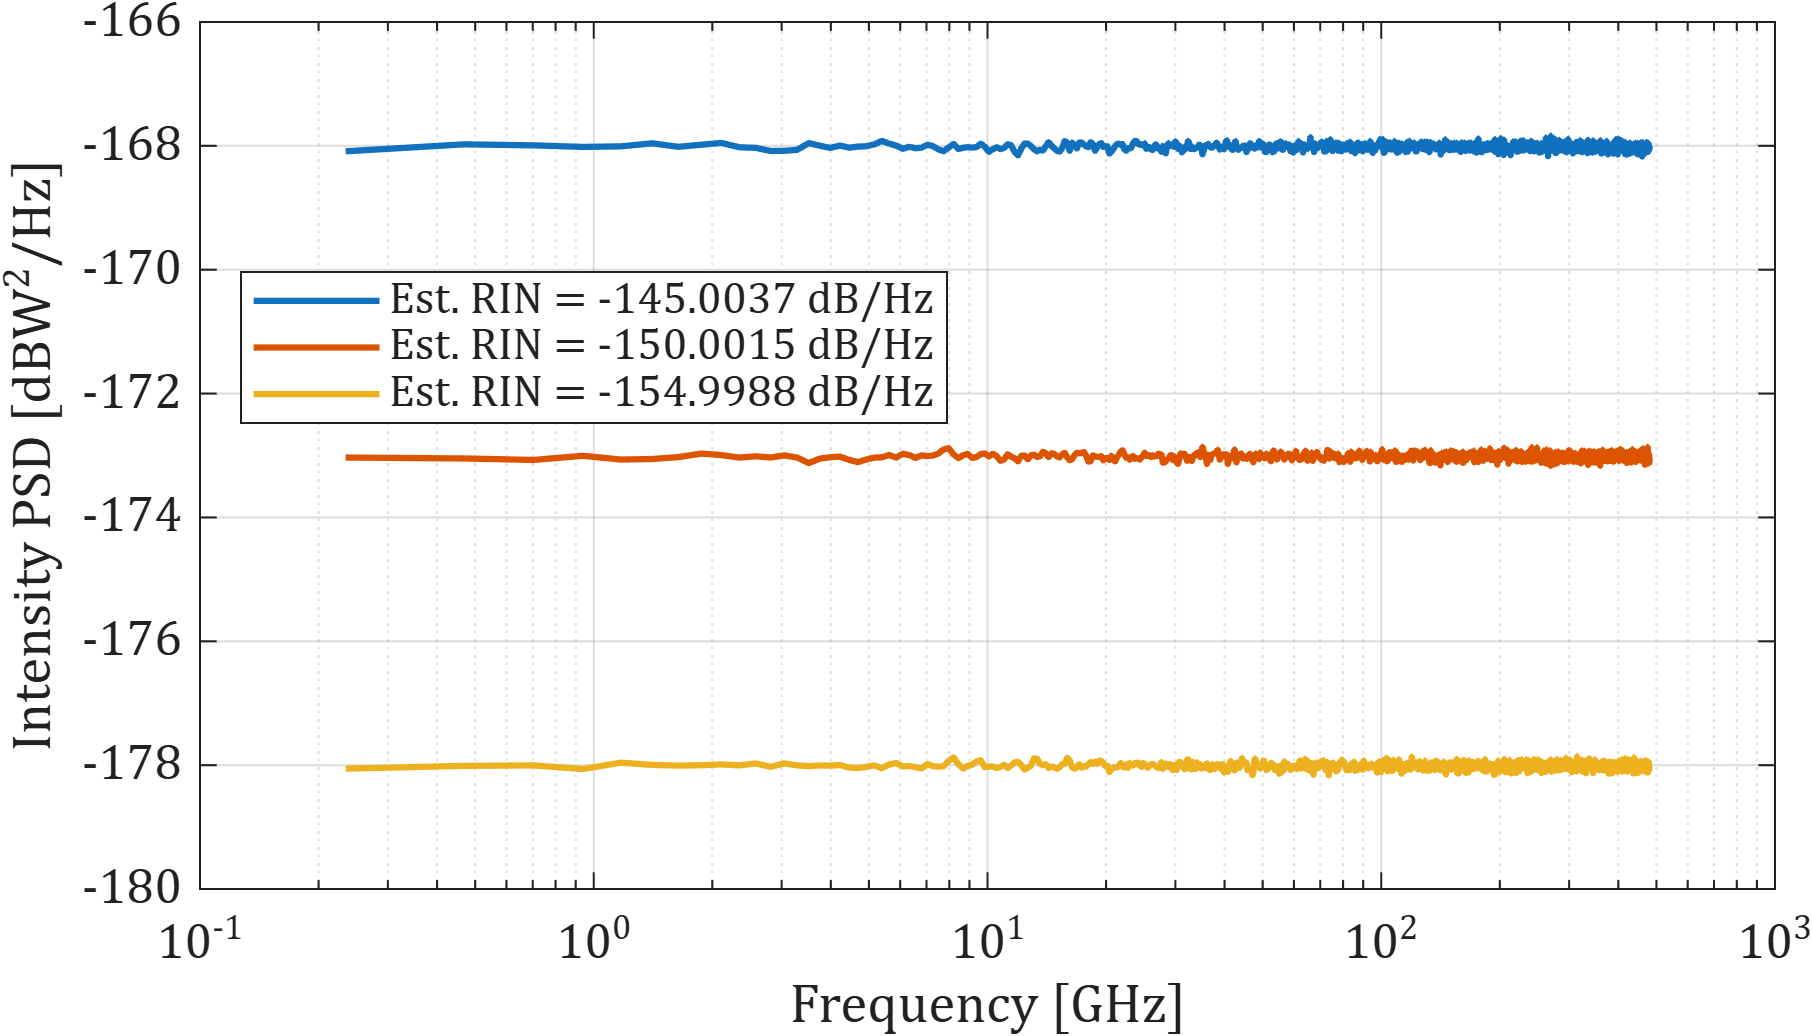
\includegraphics[width=0.7\textwidth]{figuras/ej1_rin.png}
\caption{Densidad espectral de potencia de las fluctuaciones de intensidad
para los tres valores de RIN.}
\label{fig:ej1_rin}
\end{figure}

\paragraph{Offset de frecuencia.}
El pico de la densidad espectral óptica se desplaza a la frecuencia
configurada sin modificar su forma ni su nivel
(Figura~\ref{fig:ej1_fo}). Los valores medidos, $\pm3.984$~GHz para
$FO = \pm4$~GHz, difieren del nominal en menos de un bin del estimador de
Welch ($f_s/N_{FFT} = 960\text{ GHz}/4096 = 234$~MHz): el error es de
resolución espectral y no del modelo.

\begin{figure}[H]
\centering
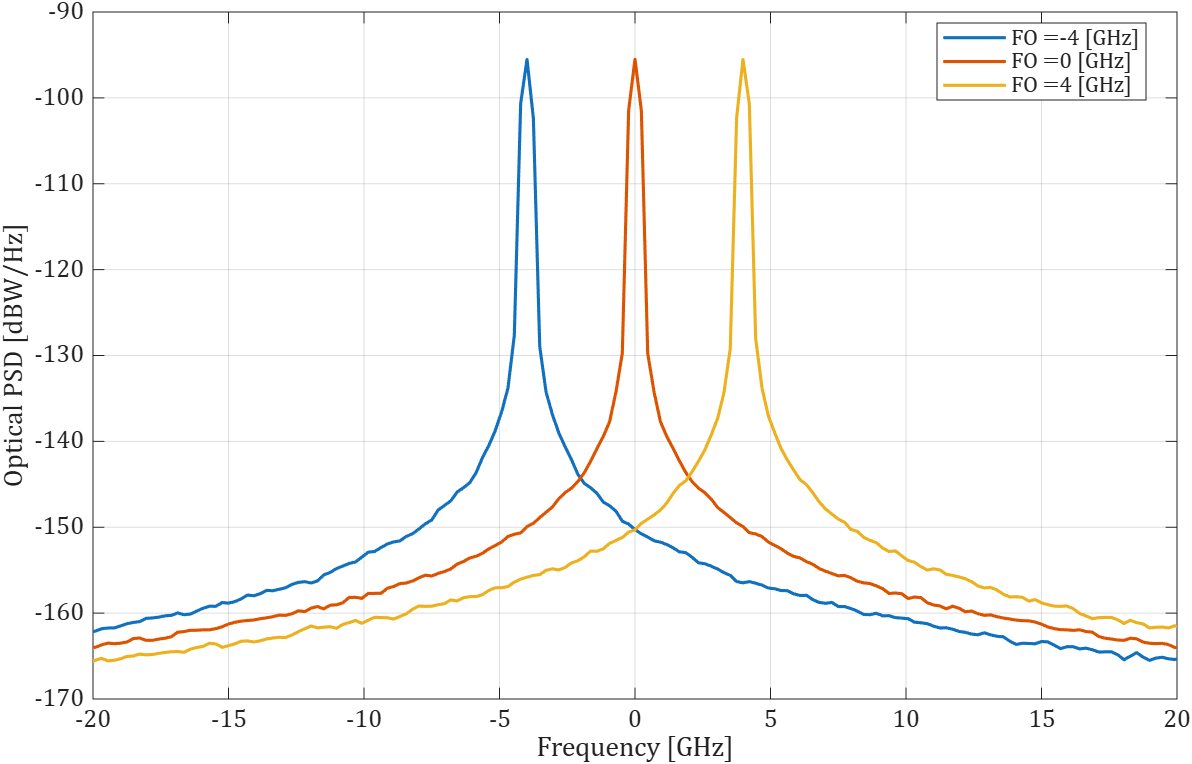
\includegraphics[width=0.7\textwidth]{figuras/ej1_fo.png}
\caption{Densidad espectral óptica para los tres valores de offset de
frecuencia.}
\label{fig:ej1_fo}
\end{figure}

\paragraph{Ruido de fase.}
Para resolver anchos de línea del orden de 100~kHz se simuló a
$f_s = 100$~MHz con $2^{21}$ muestras y una FFT de $2^{16}$ puntos
(resolución de $1.5$~kHz), promediando $16$ realizaciones por ancho de
línea. Sobre cada densidad espectral se ajustó la
ecuación~(\ref{eq:ej1_lorentz}) por mínimos cuadrados no lineales, dejando
libres la potencia y el ancho de línea (Figura~\ref{fig:ej1_psd_lw}).

\begin{table}[H]
\centering
\small
\begin{tabular}{ccc}
\toprule
$\Delta\nu$ configurado [kHz] & $\Delta\nu$ estimado [kHz] & $R^2$ del ajuste \\
\midrule
 100 &  $100.01$ & $0.9991$ \\
 300 &  $299.88$ & $0.9989$ \\
 500 &  $499.03$ & $0.9990$ \\
 700 &  $697.59$ & $0.9989$ \\
 900 &  $904.14$ & $0.9988$ \\
1100 & $1098.99$ & $0.9989$ \\
\bottomrule
\end{tabular}
\caption{Ancho de línea configurado, estimado por el ajuste lorentziano, y
coeficiente de determinación.}
\label{tab:ej1_lw}
\end{table}

\begin{figure}[H]
\centering
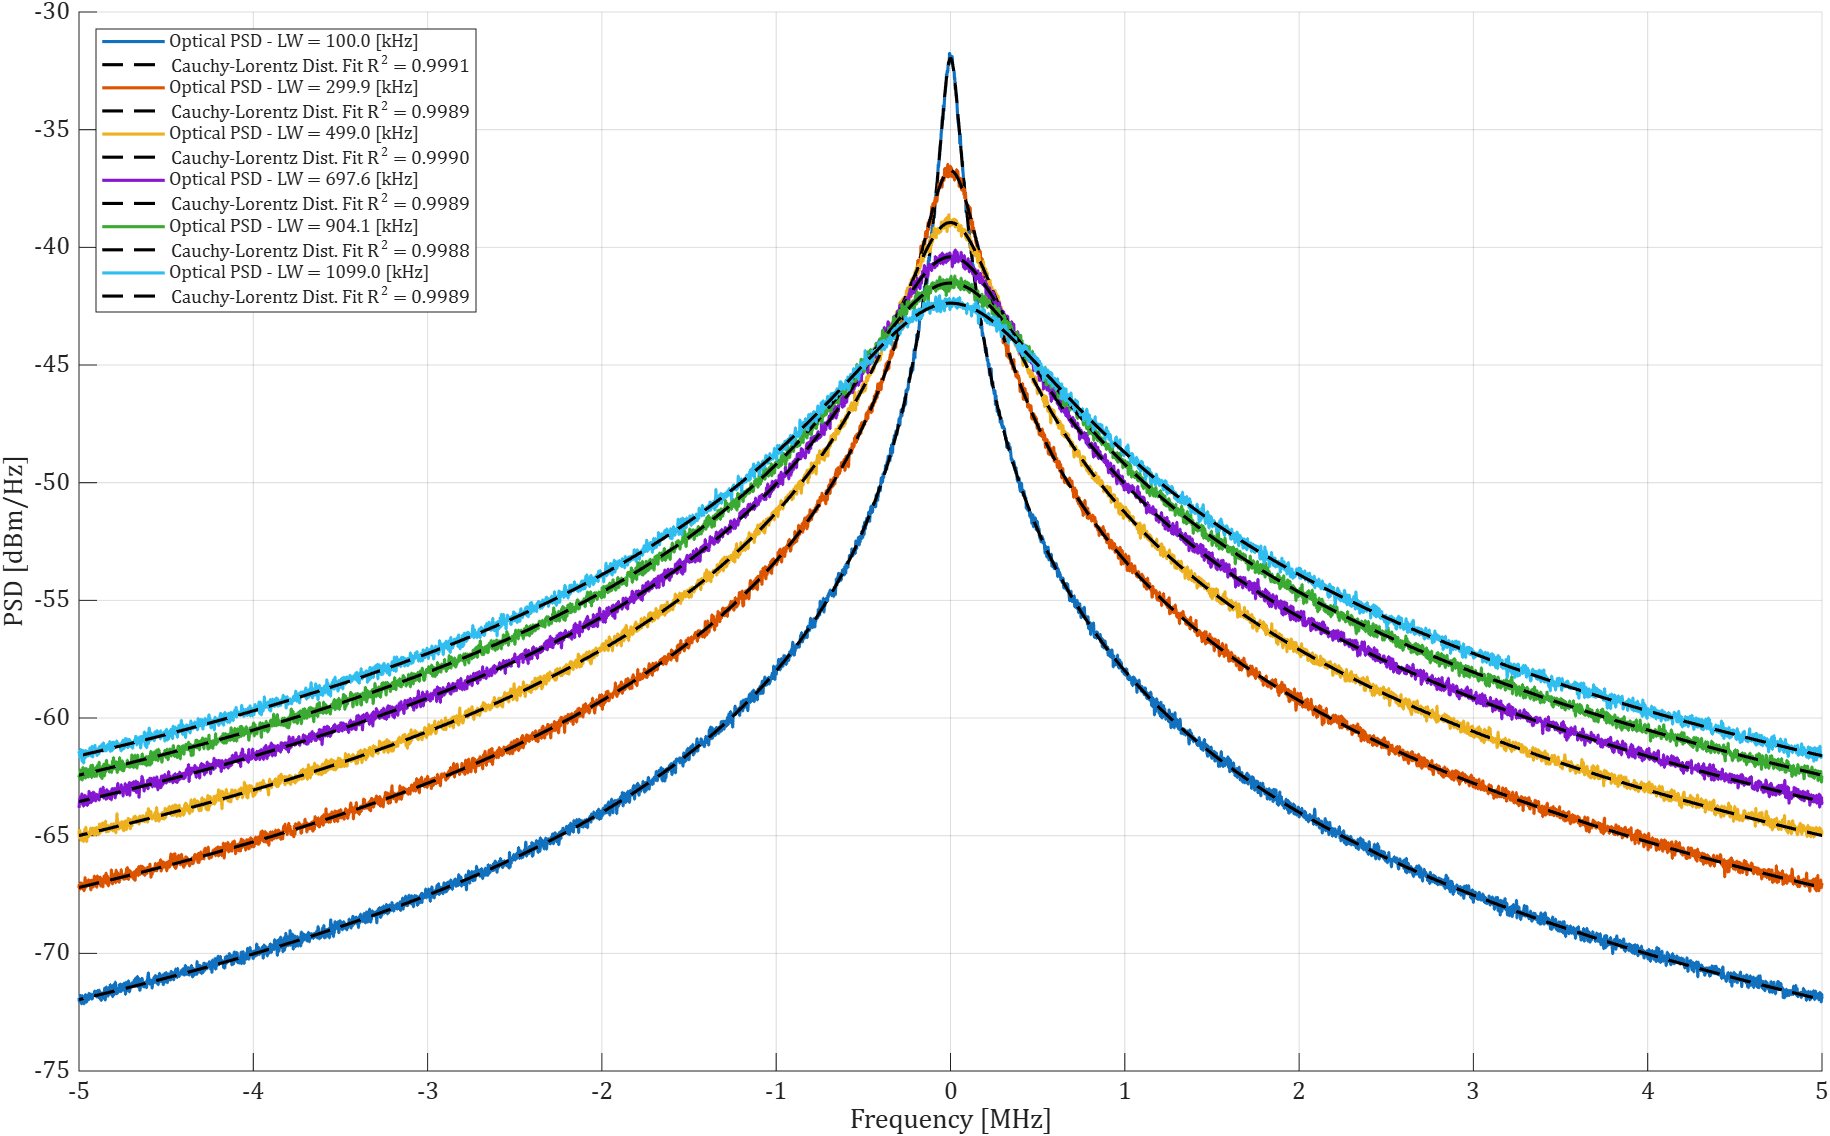
\includegraphics[width=\textwidth]{figuras/ej1_psd_lw.png}
\caption{Densidad espectral óptica simulada (color) y ajuste de
Cauchy--Lorentz (línea punteada) para cada ancho de línea.}
\label{fig:ej1_psd_lw}
\end{figure}

\begin{figure}[H]
\centering
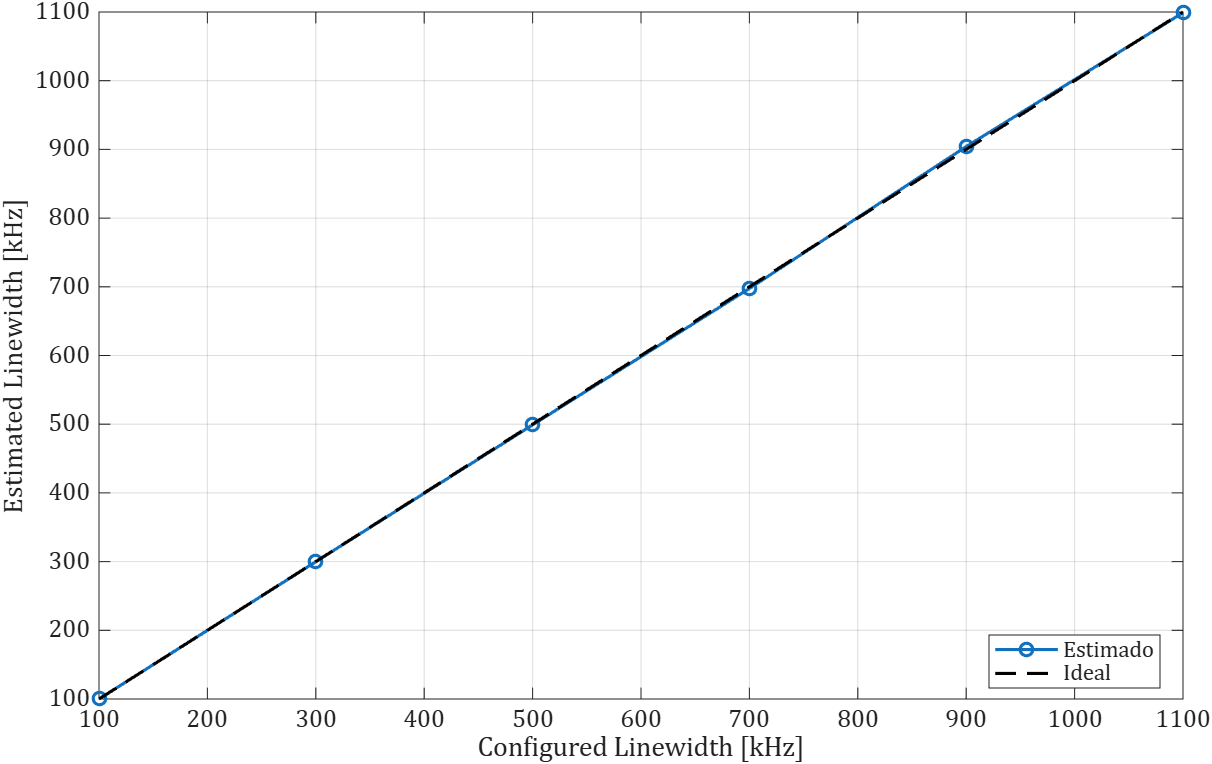
\includegraphics[width=0.7\textwidth]{figuras/ej1_lw.png}
\caption{Ancho de línea estimado en función del configurado.}
\label{fig:ej1_lw}
\end{figure}

El ancho de línea estimado sigue al configurado en todo el barrido, con
un error máximo de $0.5$~\% ($904.1$~kHz para $900$~kHz,
Figura~\ref{fig:ej1_lw}), y el ajuste lorentziano alcanza $R^2 \geq 0.9988$
en todos los casos. El residuo que queda proviene de la varianza del
estimador espectral y no de un apartamiento de la forma lorentziana: con
una sola realización ($\sim$63 segmentos promediados) el $R^2$ bajaba a
$\approx 0.98$ con el mismo modelo. Por último, a mayor ancho de línea
el pico de la densidad disminuye: la potencia total se conserva y se
reparte sobre un ancho de banda mayor, tal como predice el factor
$1/(\pi\,\Delta\nu/2)$ de la ecuación~(\ref{eq:ej1_lorentz}).

%==========================================================================
\subsection*{Ejercicio 2: Modulador MZM ideal}
%==========================================================================

El modulador Mach--Zehnder divide el campo de entrada en dos brazos mediante
un acoplador $2\times2$, aplica en cada uno un desfasaje y los recombina en
un segundo acoplador. En configuración push-pull los brazos reciben
desfasajes opuestos, $\pm\varphi$, con
%
\begin{equation}
\varphi = \frac{\pi}{2}\,\frac{V_{Bias}}{V_\pi},
\end{equation}
%
de modo que la diferencia de fase entre brazos es $\pi V_{Bias}/V_\pi$ y
$V_\pi$ es la tensión que la lleva a $\pi$. Con acopladores ideales
($K = 0.5$) el campo en el puerto de salida resulta
%
\begin{equation}
E_{out} = j\,E_{in}\cos\!\left(\frac{\pi V_{Bias}}{2V_\pi}\right),
\qquad
P_{out} = |E_{out}|^2 = P_{in}\cos^2\!\left(\frac{\pi V_{Bias}}{2V_\pi}\right).
\label{eq:ej2_mzm}
\end{equation}
%
El factor $j$ es una fase constante introducida por los acopladores y no
afecta la potencia; en las figuras de campo se lo remueve para graficar la
parte real. El segundo puerto del acoplador de salida entrega la potencia
complementaria, $P_{in}\sin^2(\cdot)$, lo que permite verificar la
conservación de la energía.

La Figura~\ref{fig:ej2_mzm} muestra el campo y la potencia normalizados en
función de $V_{Bias}/V_\pi$. La potencia tiene período $2V_\pi$ y el campo
$4V_\pi$: el campo cambia de signo al pasar por cada mínimo de potencia
($V_{Bias} = V_\pi, 3V_\pi$), mientras que la potencia, al ser su módulo
al cuadrado, no distingue ese cambio de fase de $180^\circ$.

\begin{figure}[H]
\centering
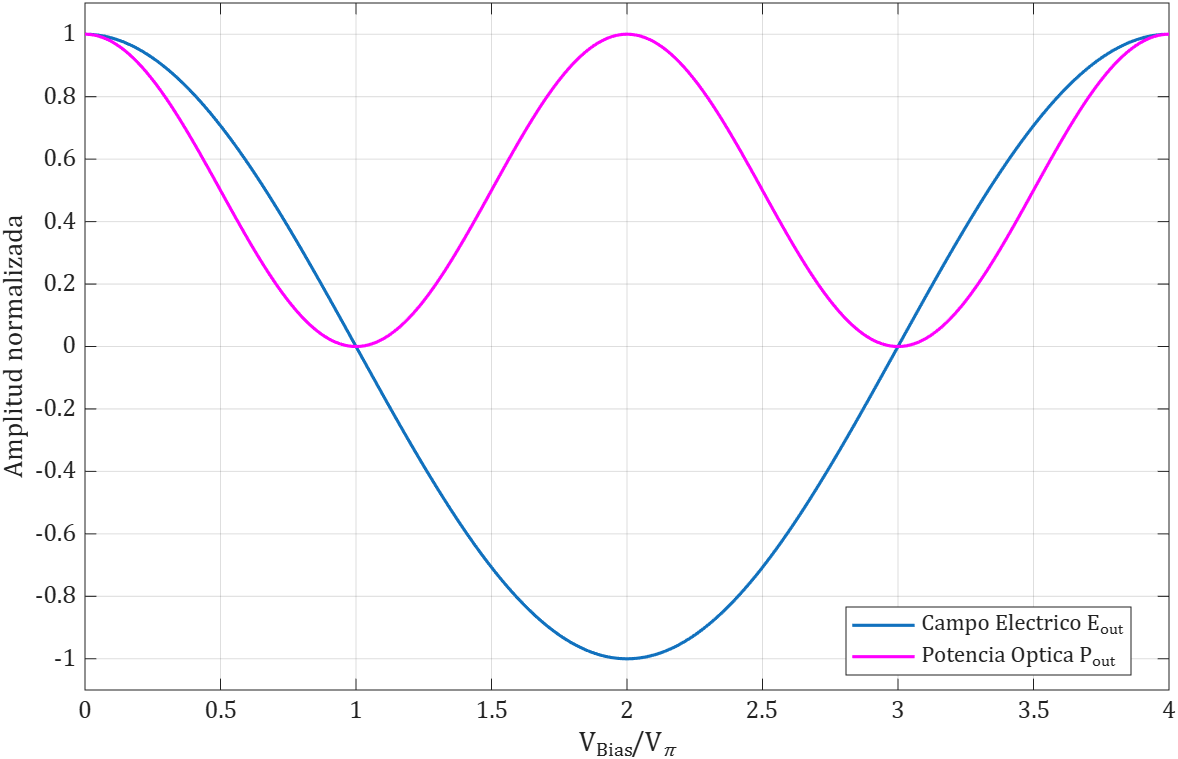
\includegraphics[width=0.75\textwidth]{figuras/ej2_mzm_ideal.png}
\caption{Campo eléctrico y potencia óptica normalizados a la salida del MZM
ideal en función de la tensión de polarización.}
\label{fig:ej2_mzm}
\end{figure}

%==========================================================================
\subsection*{Ejercicio 3: Estudio del modulador MZM}
%==========================================================================

Se excitó el MZM ideal con el láser del Ejercicio~1 ($P_0 = 20$~dBm,
$RIN = -155$~dB/Hz, $\Delta\nu = 100$~kHz) y $V_{\pi-DC} = 5$~V.

\subsubsection*{Respuesta estática}

La Figura~\ref{fig:ej3_pout} muestra la potencia de salida en ambos puertos
en función de $V_{Bias}$, con los tres puntos de polarización
característicos; la curva de campo correspondiente es la de la
Figura~\ref{fig:ej2_mzm}, escalada por $\sqrt{P_0}$.

\begin{table}[H]
\centering
\small
\begin{tabular}{lccc}
\toprule
Punto & $V_{Bias}$ [V] & $P_{out}$ [mW] & $P_{out}/P_{in}$ \\
\midrule
Máxima     & $0$           & $99.99$ & $1.000$ \\
Cuadratura & $V_\pi/2=2.5$ & $50.00$ & $0.500$ \\
Mínima     & $V_\pi=5$     & $3.8\times10^{-31}$ & $3.8\times10^{-33}$ \\
\bottomrule
\end{tabular}
\caption{Potencia de salida en los puntos de polarización ($P_{in} =
99.985$~mW).}
\label{tab:ej3_bias}
\end{table}

\begin{figure}[H]
\centering
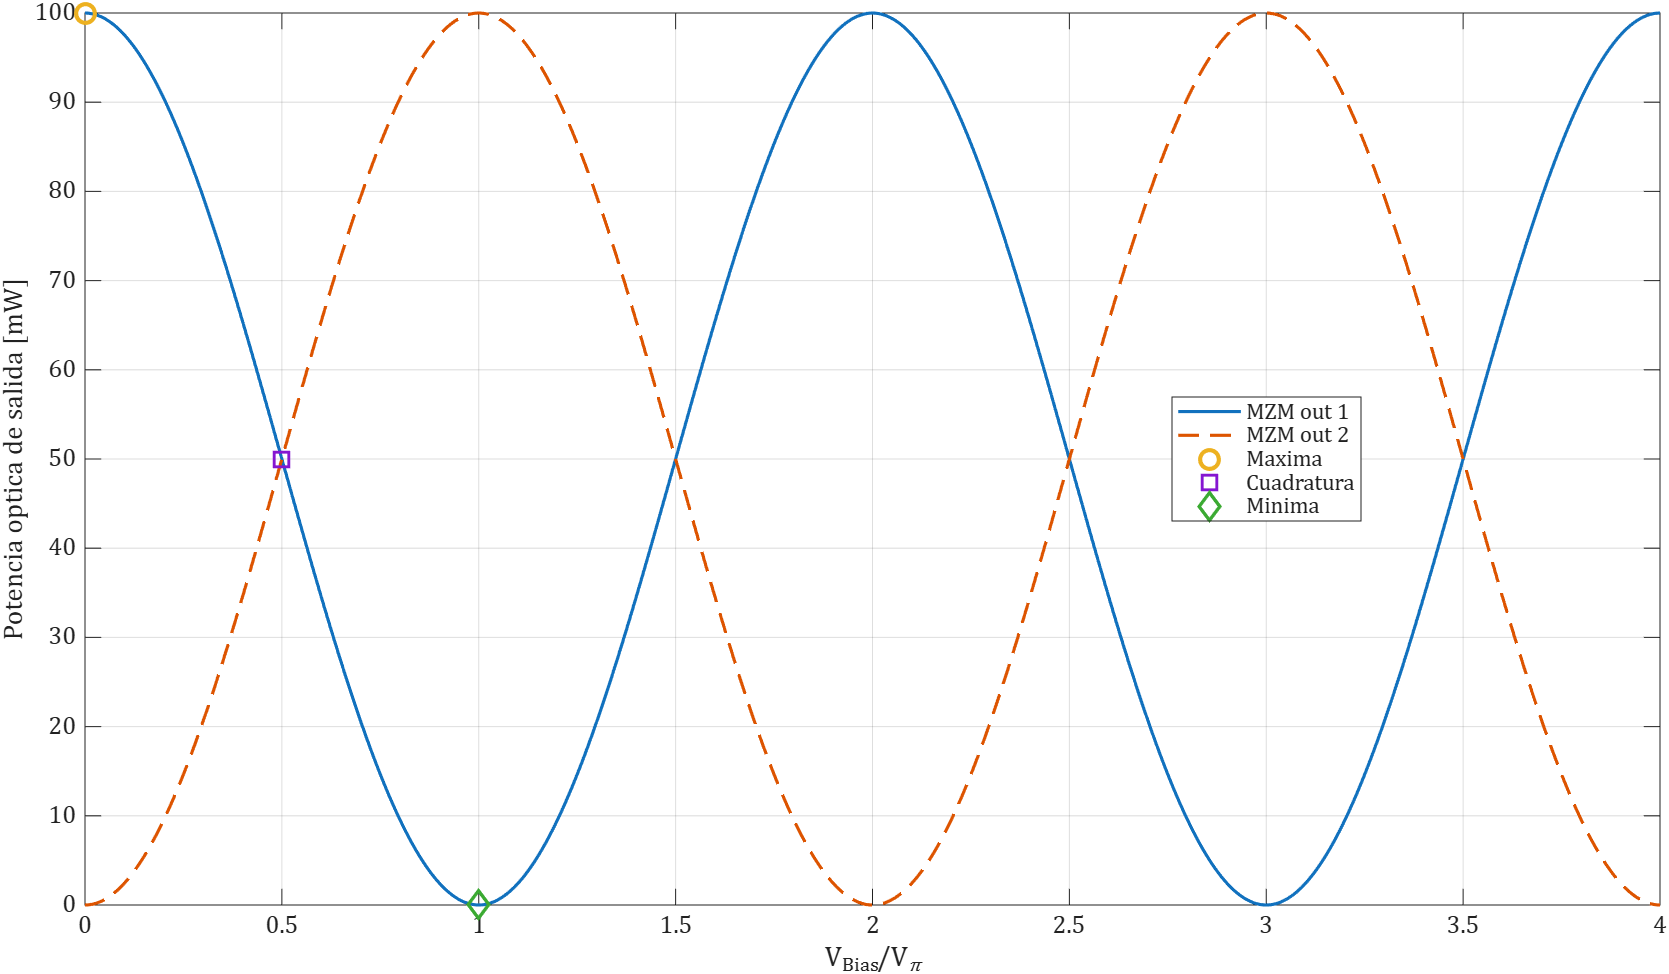
\includegraphics[width=0.8\textwidth]{figuras/ej3_pout_vbias.png}
\caption{Potencia óptica en los dos puertos de salida del MZM en función de
$V_{Bias}/V_\pi$, con los puntos de máxima, cuadratura y mínima.}
\label{fig:ej3_pout}
\end{figure}

La suma de las potencias de ambos puertos reproduce $P_{in}$ con un error
relativo máximo de $7.5\times10^{-5}$, atribuible al RIN del láser. Los
puntos de polarización cumplen roles distintos según se module potencia o
campo:
%
\begin{itemize}\itemsep2pt
\item \textbf{Cuadratura} ($V_{Bias} = V_\pi/2$): máxima pendiente de
      $P_{out}(V)$. Es el punto de operación para modulación de
      intensidad, con respuesta aproximadamente lineal en potencia.
\item \textbf{Mínima} ($V_{Bias} = V_\pi$): cruce por cero del campo, donde
      $E_{out}(V)$ tiene máxima pendiente y es aproximadamente lineal y
      bipolar. Es el punto de operación para modulación de campo,
      que es la que se usa en el modulador IQ (Ejercicios 8 a 10).
\item \textbf{Máxima} ($V_{Bias} = 0$): pendiente nula de ambas curvas; una
      señal pequeña casi no se transfiere.
\end{itemize}

\subsubsection*{Respuesta a una señal sinusoidal}

Se aplicó un tono de $80$~GHz, $v(t) = \tfrac{V_{pp}}{2}\cos(\omega_0 t)$,
con $V_{pp} = 1,\,5,\,7$~V. El campo de salida es
%
\begin{equation}
E_{out}(t) = \cos\!\left(\frac{\pi\,\big(V_{Bias} + v(t)\big)}{2V_\pi}\right),
\end{equation}
%
y el punto de polarización determina qué armónicos aparecen, según la
simetría de la curva de transferencia alrededor de ese punto:
%
\begin{itemize}\itemsep2pt
\item En \textbf{máxima} ($V_{Bias} = 0$) el campo es
      $\cos\!\big(\pi v/2V_\pi\big)$, una función par de la señal:
      $+v$ y $-v$ producen la misma salida. La salida se repite cada medio
      período de la sinusoide, por lo que sólo contiene la continua y los
      armónicos pares; no hay componente en $80$~GHz.
\item En \textbf{mínima} ($V_{Bias} = V_\pi$) el campo es
      $-\sin\!\big(\pi v/2V_\pi\big)$, una función impar: al cambiar
      el signo de la señal cambia el signo de la salida. Sólo contiene los
      armónicos impares y desaparece la continua.
\item En \textbf{cuadratura} ($V_{Bias} = V_\pi/2$) la curva no tiene
      ninguna de las dos simetrías y aparecen todos los armónicos.
\end{itemize}
%
La Tabla~\ref{tab:ej3_armonicos} resume los niveles medidos sobre el
espectro del campo, que confirman ese comportamiento.

\begin{table}[H]
\centering
\small
\begin{tabular}{lcccc}
\toprule
Punto & $V_{pp}$ [V] & $80$ GHz & $160$ GHz & $240$ GHz \\
\midrule
Máxima     & 1 & ---     & $-51.0$ & --- \\
           & 5 & ---     & $-21.9$ & --- \\
           & 7 & ---     & $-15.1$ & --- \\
\midrule
Cuadratura & 1 & $-22.7$ & $-51.0$ & --- \\
           & 5 & $-8.0$  & $-21.9$ & $-38.9$ \\
           & 7 & $-4.3$  & $-15.1$ & $-29.0$ \\
\midrule
Mínima     & 1 & $0$     & ---     & $-59.4$ \\
           & 5 & $0$     & ---     & $-30.9$ \\
           & 7 & $0$     & ---     & $-24.7$ \\
\bottomrule
\end{tabular}
\caption{Nivel de cada armónico del campo en dB, relativo a la componente
más fuerte (la continua en máxima y cuadratura, la fundamental en mínima).
``---'' indica una componente por debajo del piso de ruido de la simulación
($\approx -72$~dB).}
\label{tab:ej3_armonicos}
\end{table}

\begin{figure}[H]
\centering
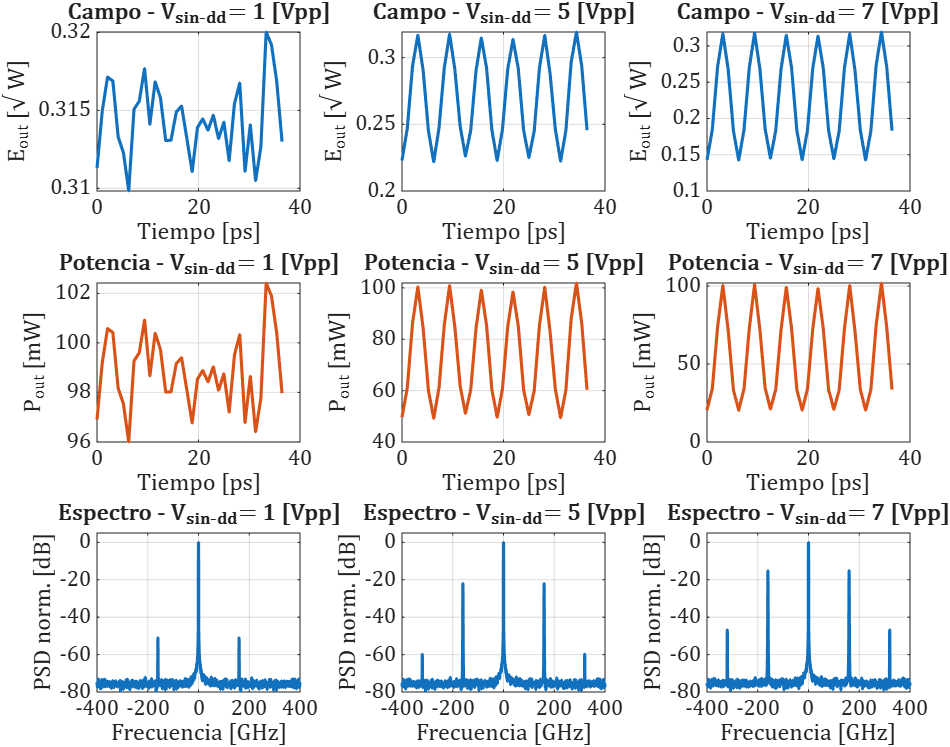
\includegraphics[width=\textwidth]{figuras/ej3_sin_maxima.png}
\caption{Campo eléctrico (arriba), potencia óptica (centro) y espectro del
campo (abajo) con el MZM polarizado en \textbf{máxima}.}
\label{fig:ej3_max}
\end{figure}

\paragraph{Máxima.} Para $1$~V$_{pp}$ la excursión permanece en la zona de
pendiente nula: la potencia varía como máximo un $2.5$~\%
($1-\cos^2(\pi\cdot0.5/10)$), del mismo orden que las fluctuaciones del
RIN (Figura~\ref{fig:ej3_max}). Al crecer la
amplitud la salida se vuelve periódica, pero al doble de la frecuencia de
excitación: la señal recorre el máximo de la curva hacia ambos lados y cada
semiciclo produce la misma variación. Es la duplicación de frecuencia que
corresponde a la ausencia de armónicos impares.

\begin{figure}[H]
\centering
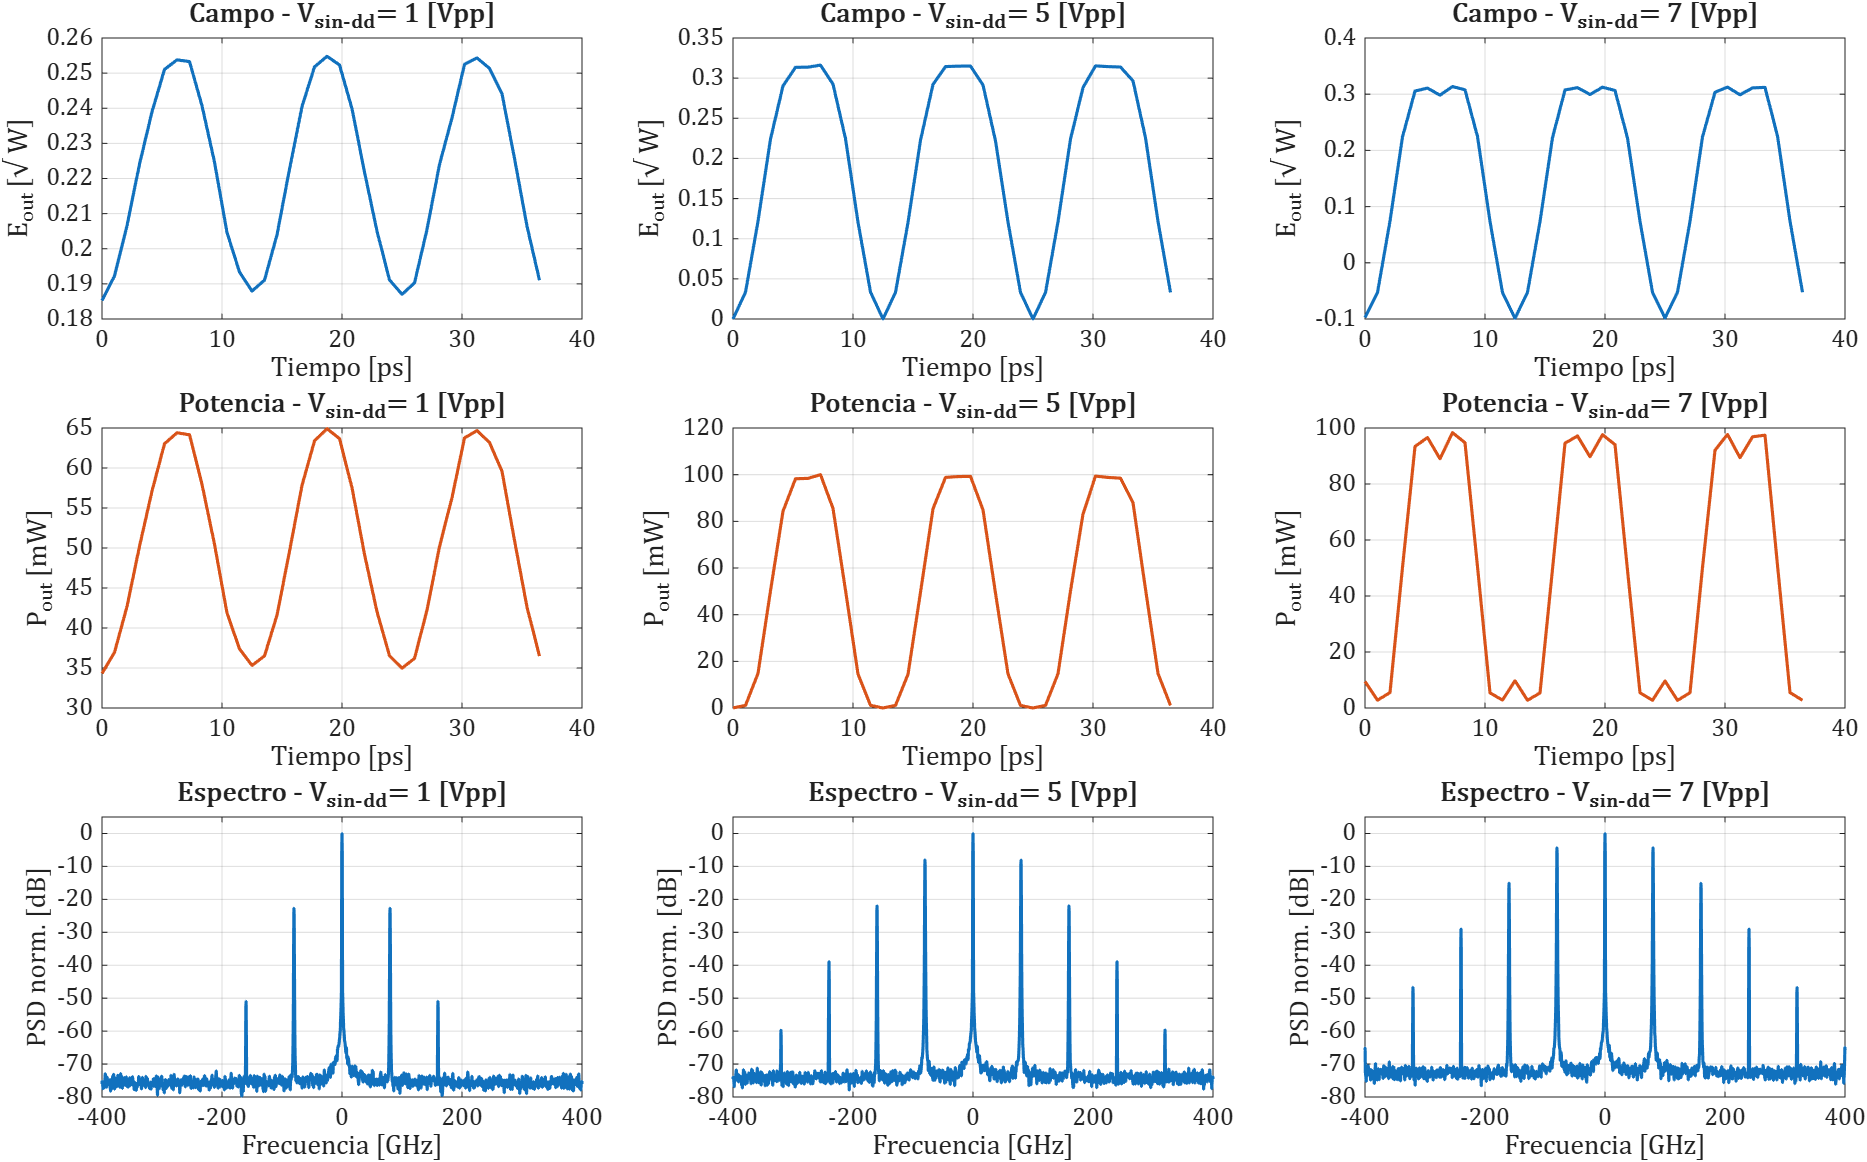
\includegraphics[width=\textwidth]{figuras/ej3_sin_cuadratura.png}
\caption{Campo eléctrico (arriba), potencia óptica (centro) y espectro del
campo (abajo) con el MZM polarizado en \textbf{cuadratura}.}
\label{fig:ej3_cuad}
\end{figure}

\paragraph{Cuadratura.} Para $1$~V$_{pp}$ la respuesta es prácticamente
lineal: el segundo armónico está $28$~dB por debajo de la fundamental
(Figura~\ref{fig:ej3_cuad}). Al aumentar la amplitud crece la distorsión y
para $7$~V$_{pp}$ el segundo y tercer armónico quedan a sólo $11$ y
$25$~dB de la fundamental. La continua domina el espectro en todos los
casos: en cuadratura se transmite en promedio la mitad de la potencia
incidente como portadora, independientemente de la señal.

\begin{figure}[H]
\centering
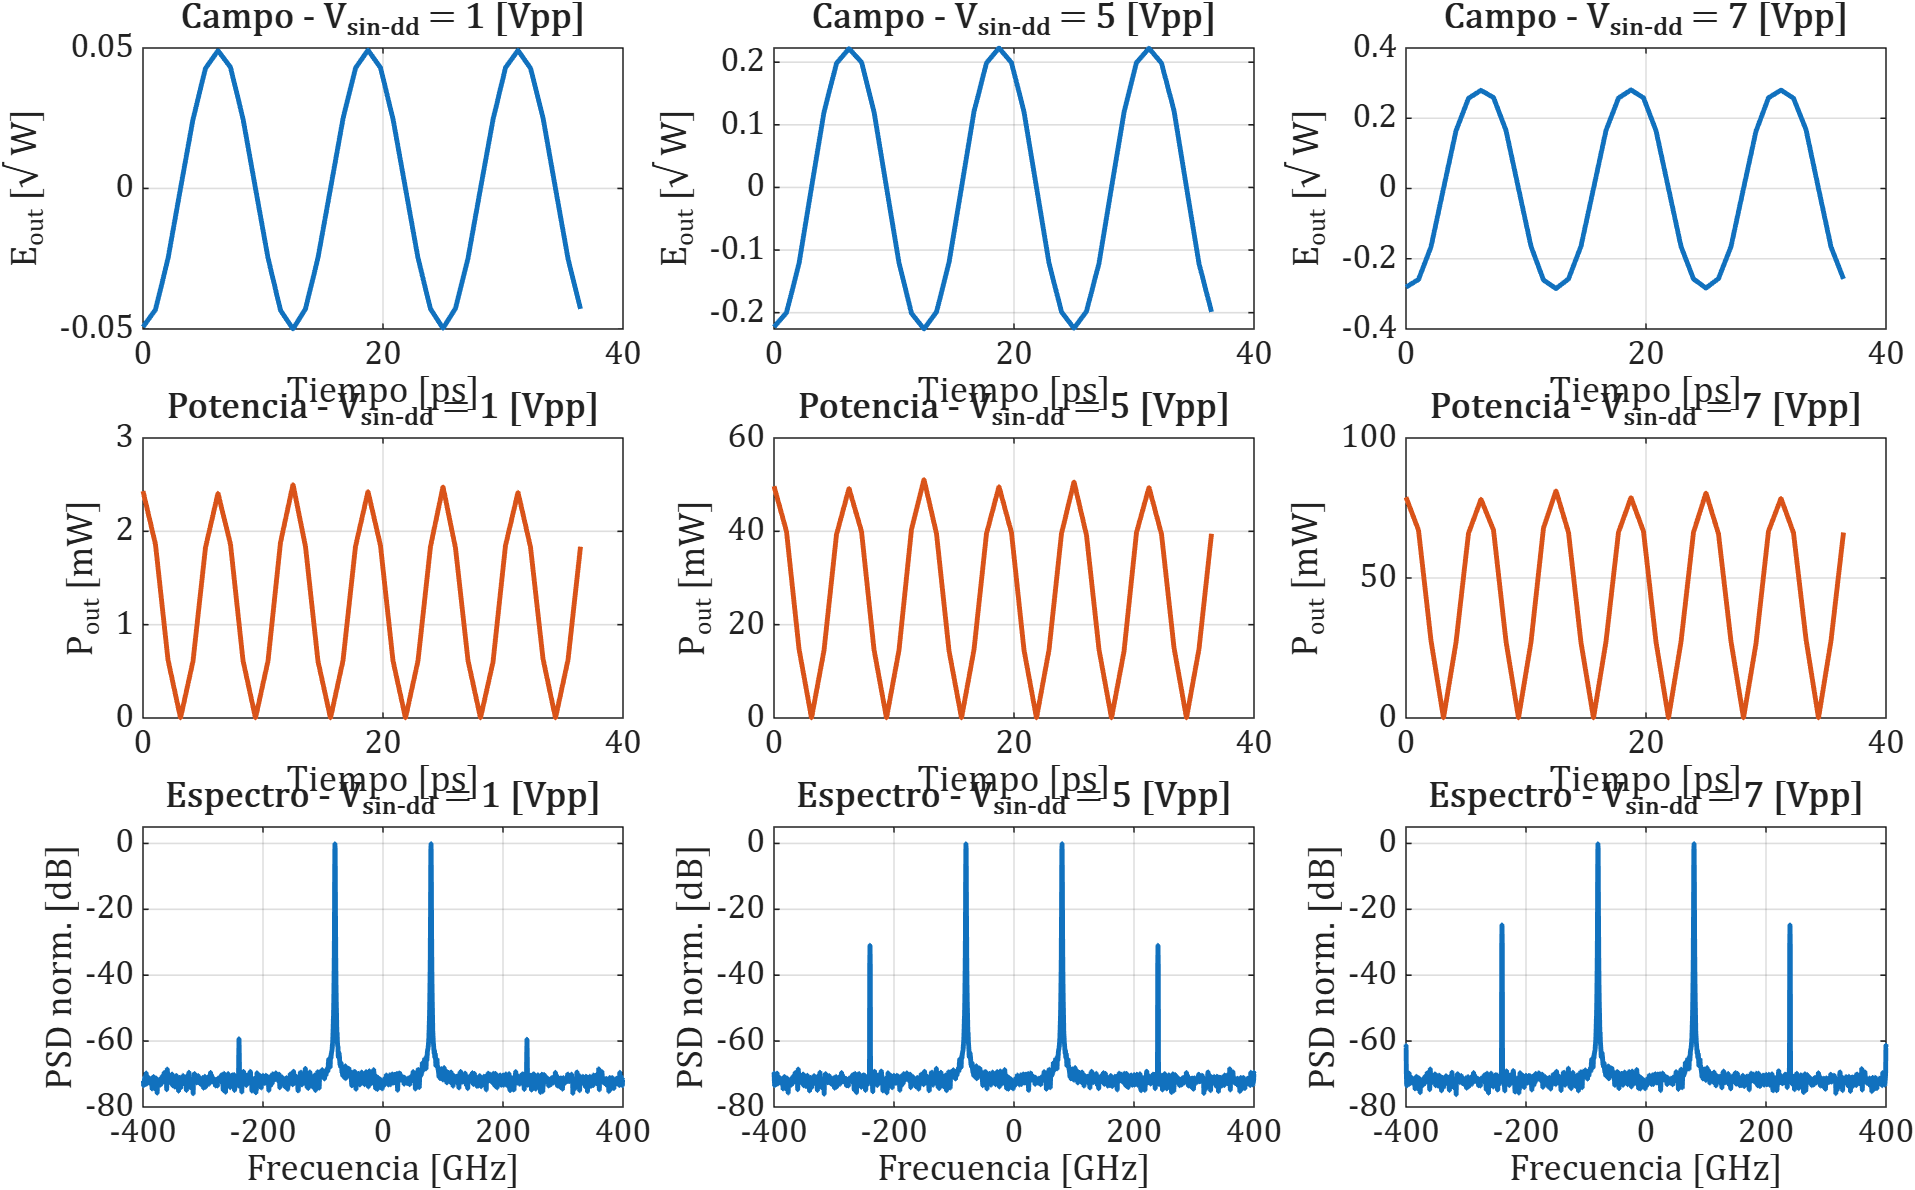
\includegraphics[width=\textwidth]{figuras/ej3_sin_minima.png}
\caption{Campo eléctrico (arriba), potencia óptica (centro) y espectro del
campo (abajo) con el MZM polarizado en \textbf{mínima}.}
\label{fig:ej3_min}
\end{figure}

\paragraph{Mínima.} El campo reproduce la sinusoide con signo (es una
modulación bipolar) y sin portadora (Figura~\ref{fig:ej3_min}). La única
distorsión es el tercer armónico, que para $1$~V$_{pp}$ está a
$-59$~dB y aún para $7$~V$_{pp}$ se mantiene a $-25$~dB. Es el punto de
mayor linealidad en campo, aunque su potencia oscila al doble de la
frecuencia de la señal.

%==========================================================================
\subsection*{Ejercicio 4: Modelo de un modulador MZM con desperfectos}
%==========================================================================

\subsubsection*{Implementación}

\paragraph{Extinction ratio.}
Siguiendo la consigna, el desperfecto de fabricación de los acopladores se
incorpora en su factor de acoplamiento,
%
\begin{equation}
K_c = K\,(1-\alpha), \qquad \alpha = 10^{-ER[\text{dB}]/20}.
\end{equation}
%
Con $K_c \neq 0.5$ los dos brazos dejan de tener la misma amplitud, de modo
que en el punto de mínima la interferencia destructiva ya no es completa y
queda un campo residual de amplitud relativa $\alpha$. El cociente entre la
potencia máxima y la mínima resulta entonces $1/\alpha^2$, es decir, el
$ER$ especificado.

\paragraph{Pérdida de inserción.}
Las pérdidas de propagación y scattering se modelan como una
atenuación de $IL$~dB a la entrada del modulador:
$E_{in} \rightarrow E_{in}/10^{IL/20}$.

\subsubsection*{Resultados}

Se utilizó $V_{\pi-DC} = 5$~V, $ER = 25$~dB e $IL = 4$~dB, con el mismo láser
del Ejercicio~3. Las Figuras~\ref{fig:ej4_pout} y~\ref{fig:ej4_eout}
muestran la potencia y el campo de salida en función de $V_{Bias}$.

\begin{figure}[H]
\centering
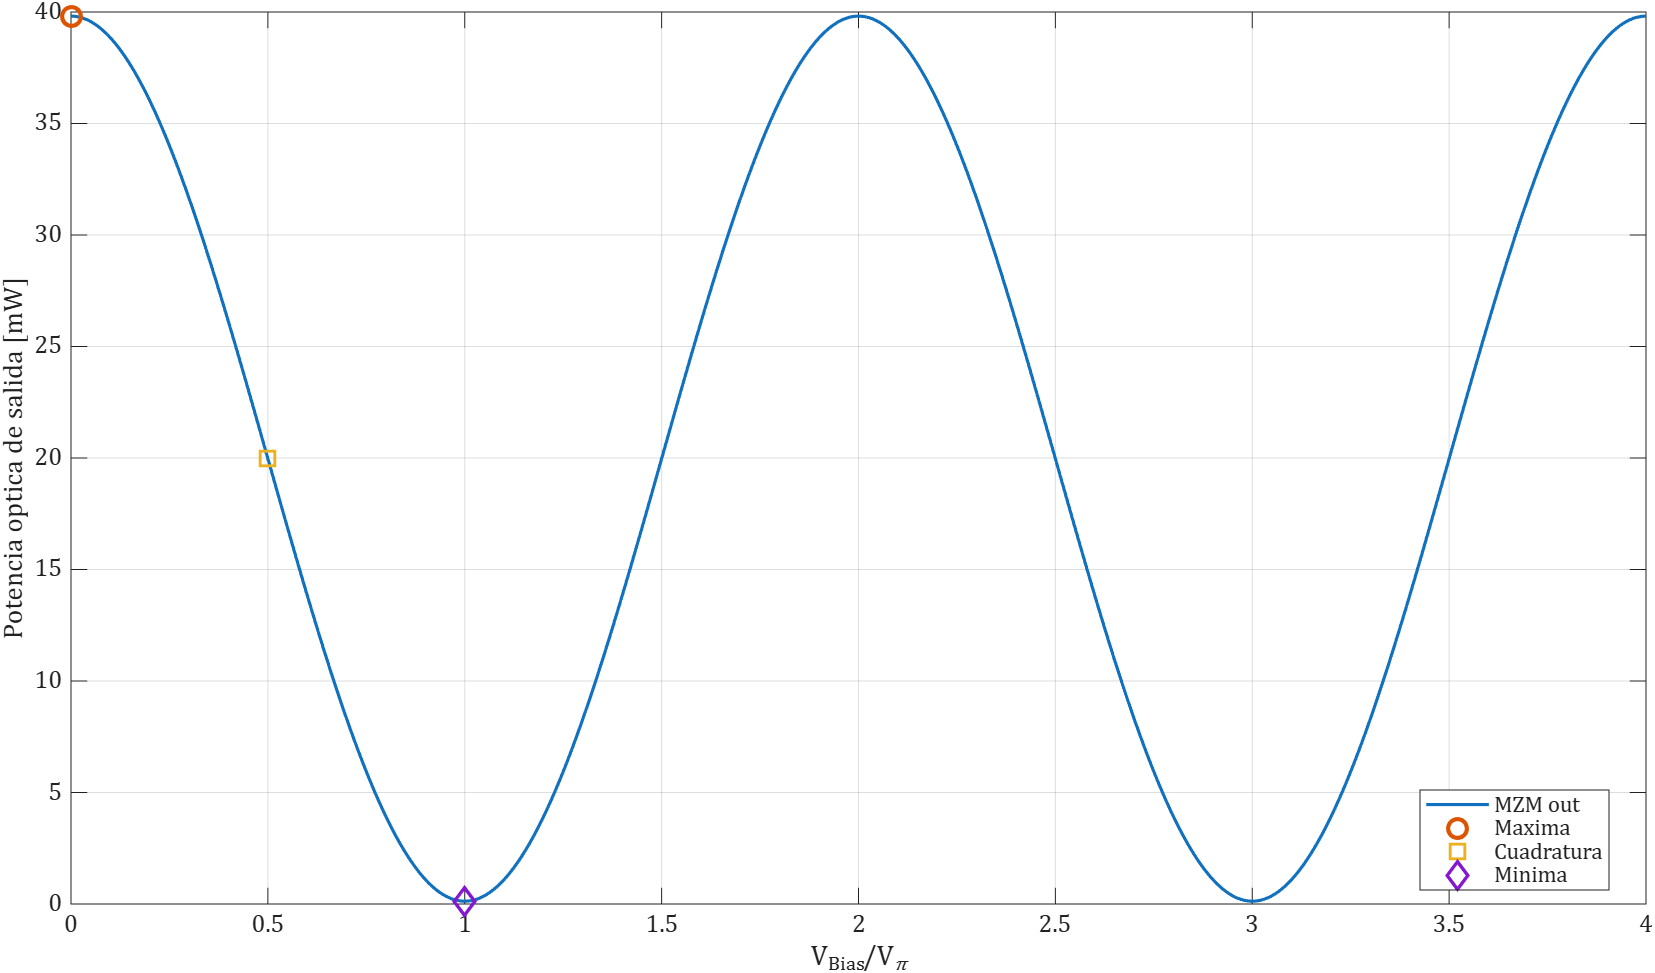
\includegraphics[width=0.75\textwidth]{figuras/ej4_pout_vbias.png}
\caption{Potencia óptica de salida del MZM con $ER = 25$~dB e $IL = 4$~dB.}
\label{fig:ej4_pout}
\end{figure}

\begin{figure}[H]
\centering
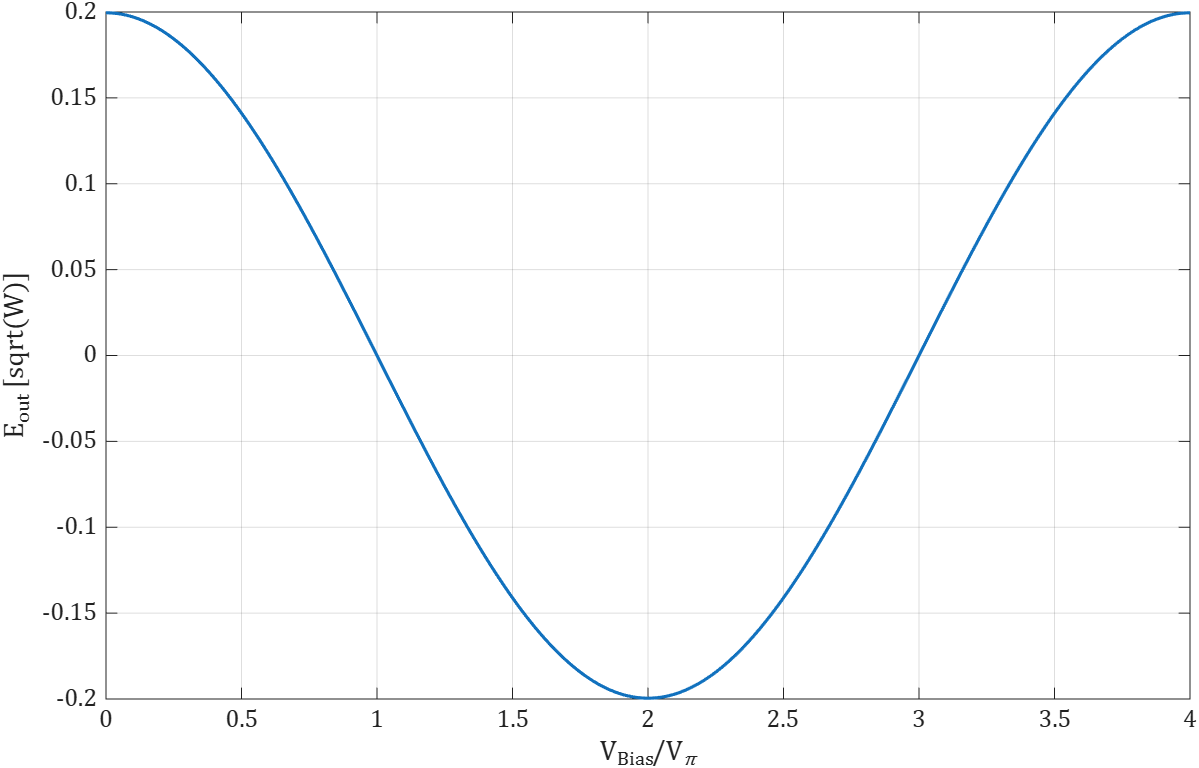
\includegraphics[width=0.75\textwidth]{figuras/ej4_eout_vbias.png}
\caption{Campo eléctrico de salida del MZM con $ER = 25$~dB e $IL = 4$~dB.}
\label{fig:ej4_eout}
\end{figure}

En escala lineal ambas curvas son prácticamente idénticas a las del MZM
ideal escaladas por la pérdida de inserción: con $ER = 25$~dB la potencia
en mínima es sólo el $0.3$~\% de la máxima. La curva de campo de la
Figura~\ref{fig:ej4_eout} es la componente en fase con el láser, que sigue
cruzando por cero; el campo residual de mínima queda en cuadratura de fase
y por eso sólo se manifiesta en la potencia.

Para visualizar el efecto se repitió la simulación con $ER = 9$~dB
(Figura~\ref{fig:ej4_norm}): la potencia ya no llega a cero y en
$V_{Bias} = V_\pi$ queda en $0.126$ de la máxima. En escala logarítmica
(Figura~\ref{fig:ej4_dbm}) el piso se aprecia también con el valor pedido
por la consigna: para $ER = 25$~dB la potencia en mínima queda en
$-9.0$~dBm ($0.126$~mW) en lugar de caer indefinidamente.

\begin{figure}[H]
\centering
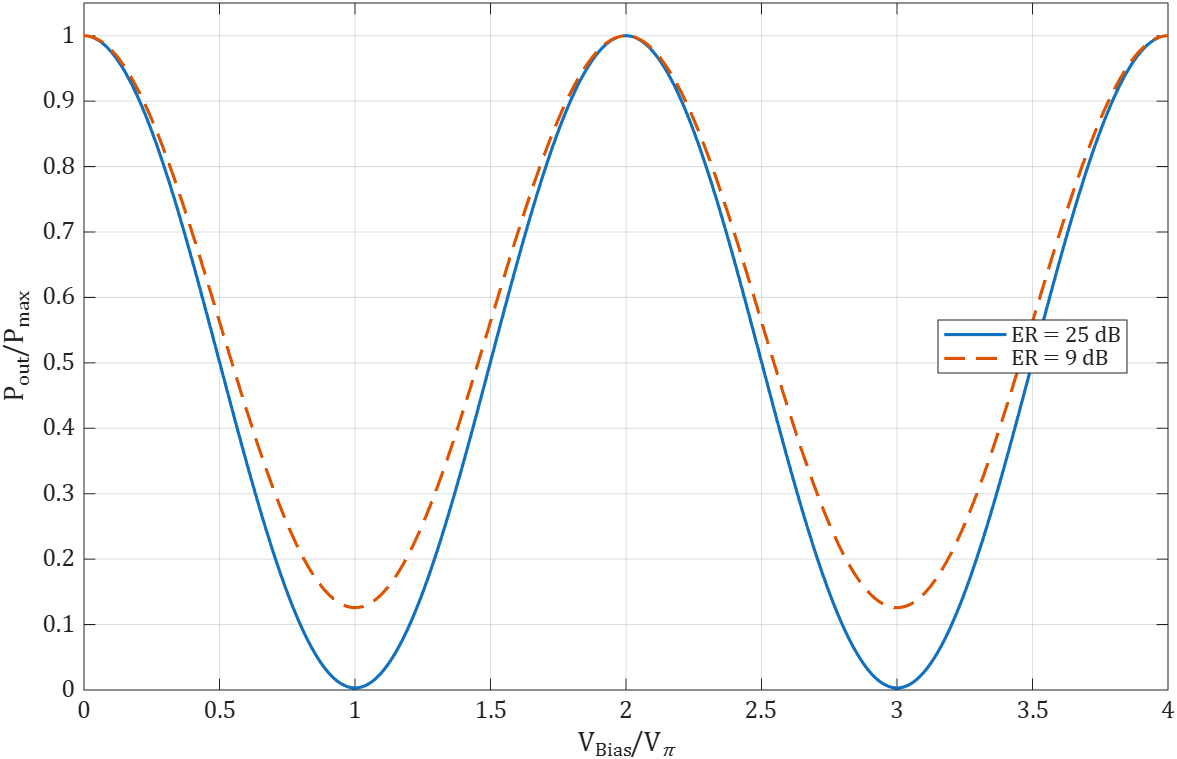
\includegraphics[width=0.75\textwidth]{figuras/ej4_pout_norm.png}
\caption{Potencia de salida normalizada para $ER = 25$~dB y $ER = 9$~dB.}
\label{fig:ej4_norm}
\end{figure}

\begin{figure}[H]
\centering
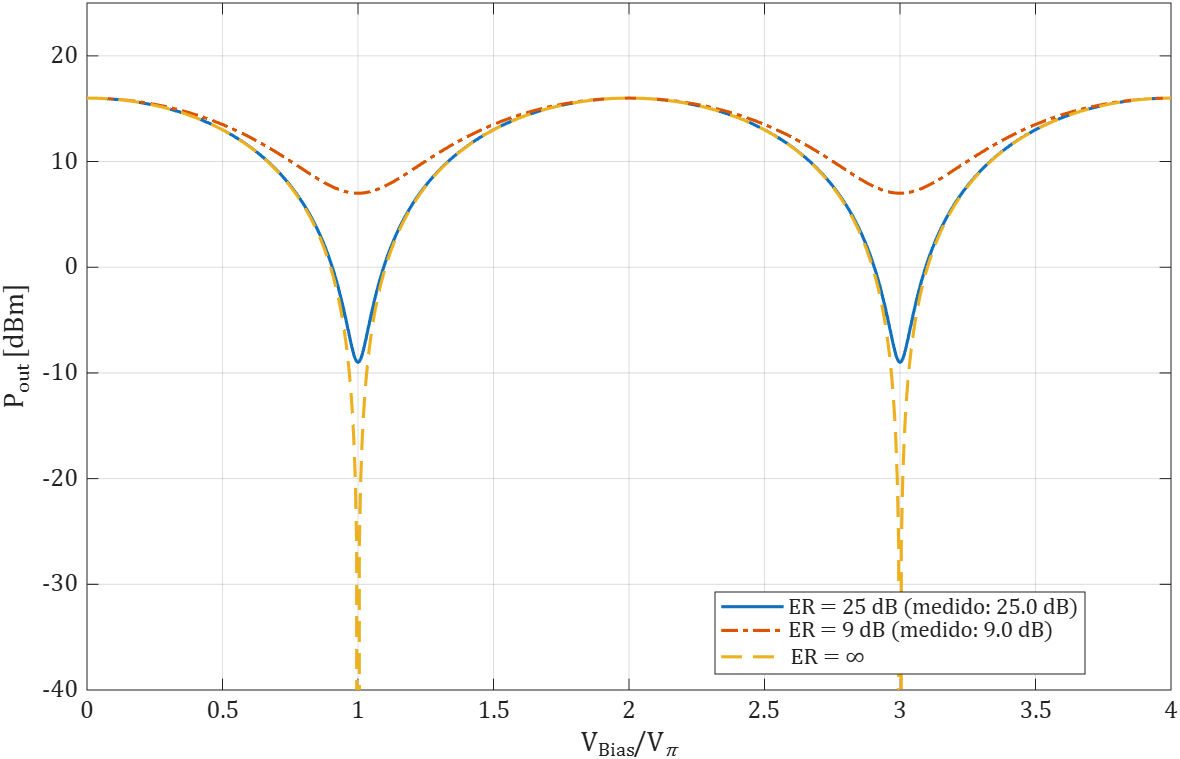
\includegraphics[width=0.75\textwidth]{figuras/ej4_pout_dbm.png}
\caption{Potencia de salida en dBm para $ER = 25$~dB, $ER = 9$~dB y para el
MZM ideal ($ER = \infty$), con $IL = 4$~dB.}
\label{fig:ej4_dbm}
\end{figure}

\paragraph{c) Pérdida en el punto de máxima.}
Con $P_{in} = 100.01$~mW y $P_{out,max} = 39.81$~mW:
%
\begin{equation}
10\log_{10}\!\left(\frac{P_{in}}{P_{out,max}}\right) = 4.00\ \text{dB}.
\end{equation}
%
Esta cuenta mide la \textbf{pérdida de inserción} ($IL$) del modulador: en
máxima la interferencia es constructiva y la única pérdida es la de las
guías de onda, que coincide con los $4$~dB configurados.

\paragraph{Verificación del ER.}
El cociente entre la potencia en máxima y en mínima reproduce el valor
configurado en los dos casos simulados (Tabla~\ref{tab:ej4_er}).

\begin{table}[H]
\centering
\small
\begin{tabular}{cccc}
\toprule
$ER$ configurado [dB] & $P_{out,max}$ [mW] & $P_{out,min}$ [mW] & $ER$ medido [dB] \\
\midrule
$25$ & $39.81$ & $0.126$ & $25.00$ \\
$9$  & $39.81$ & $5.01$  & $9.00$ \\
\bottomrule
\end{tabular}
\caption{Relación de extinción medida como
$10\log_{10}(P_{out,max}/P_{out,min})$.}
\label{tab:ej4_er}
\end{table}

En resumen, ambos desperfectos actúan sobre regiones distintas de la
curva: la pérdida de inserción desplaza toda la curva hacia abajo en
$IL$~dB y se mide en el punto de máxima, mientras que el ER finito sólo
limita la profundidad del mínimo y se mide como el cociente entre máxima y
mínima.

%==========================================================================
\subsection*{Ejercicio 5: Pérdidas de potencia con señal PAM4}
%==========================================================================
% Figuras y datos: tests/test_MZM_ex5.m

\subsubsection*{Configuración}

Se mantuvieron las condiciones del Ejercicio~4 (láser de $20$~dBm,
$V_\pi = 5$~V, $ER = 25$~dB, $IL = 4$~dB) y se inyectó al modulador una
señal PAM4 con pulso de coseno realzado de roll-off $0.2$, a $240$~Gbaud y
muestreada a $f_s = 960$~GHz (4 muestras por símbolo).

Los $2$~V$_{pp}$ se tomaron sobre la forma de onda completa, incluyendo el
sobrepico que el pulso de coseno realzado produce entre símbolos. Con ese
criterio los cuatro niveles de símbolo quedan en $\pm0.551$~V y
$\pm0.184$~V (Figura~\ref{fig:ej5_entrada}). Los diagramas de ojo se
dibujan sobre una ventana de dos símbolos con el instante de muestreo en el
centro; la señal se interpola únicamente para graficar, sin intervenir en
ningún cálculo.

\begin{figure}[H]
\centering
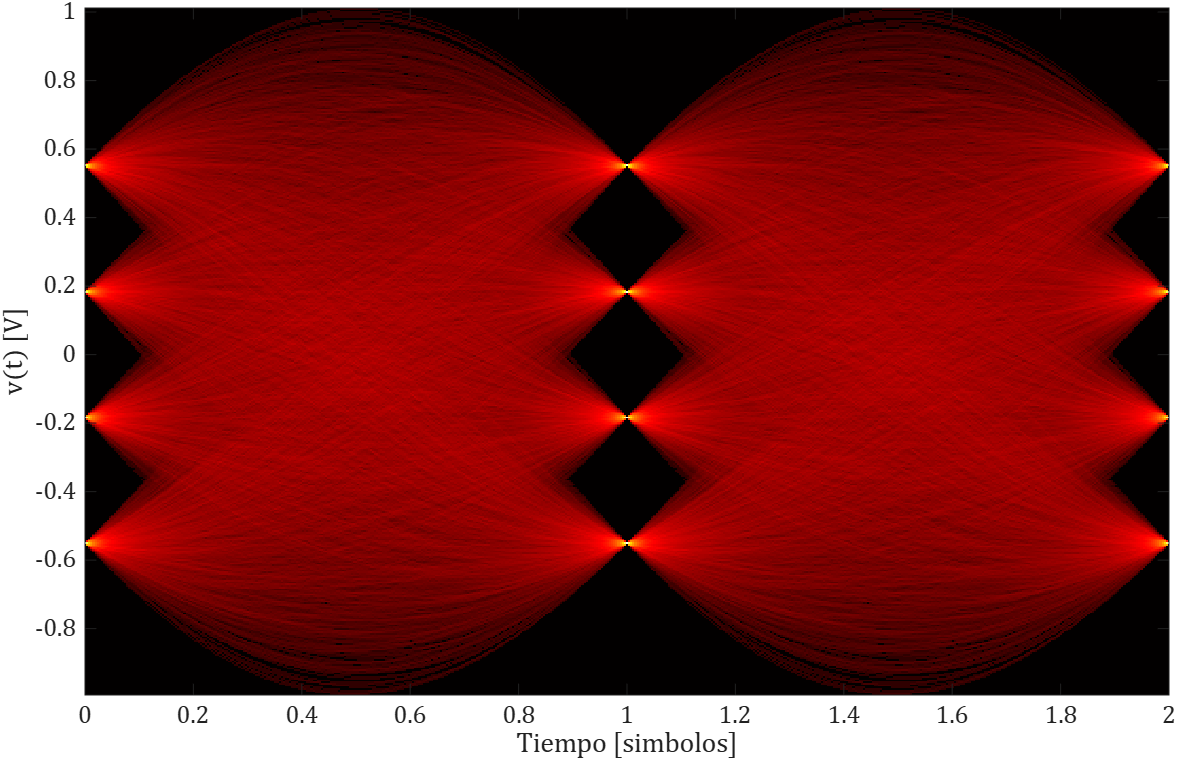
\includegraphics[width=0.6\textwidth]{figuras/ej5_ojo_entrada.png}
\caption{Diagrama de ojo de la señal eléctrica PAM4 a la entrada del
modulador ($2$~V$_{pp}$).}
\label{fig:ej5_entrada}
\end{figure}

\subsubsection*{Resultados}

La pérdida de potencia se calculó como
$10\log_{10}(P_{in}/\langle P_{out}\rangle)$, con $\langle P_{out}\rangle$
la potencia óptica media a la salida (Tabla~\ref{tab:ej5_perdidas}). La
Figura~\ref{fig:ej5_ojos} muestra los diagramas de ojo del campo y de la
potencia en los tres puntos de polarización.

\begin{table}[H]
\centering
\small
\begin{tabular}{lccc}
\toprule
Punto & $V_{Bias}$ [V] & $\langle P_{out}\rangle$ [mW] & Pérdida [dB] \\
\midrule
Máxima     & $0$   & $39.20$ & $4.07$ \\
Cuadratura & $2.5$ & $19.99$ & $6.99$ \\
Mínima     & $5$   & $0.739$ & $21.31$ \\
\bottomrule
\end{tabular}
\caption{Potencia media de salida y pérdida de potencia en cada punto de
polarización ($P_{in} = 100$~mW).}
\label{tab:ej5_perdidas}
\end{table}

\begin{figure}[H]
\centering
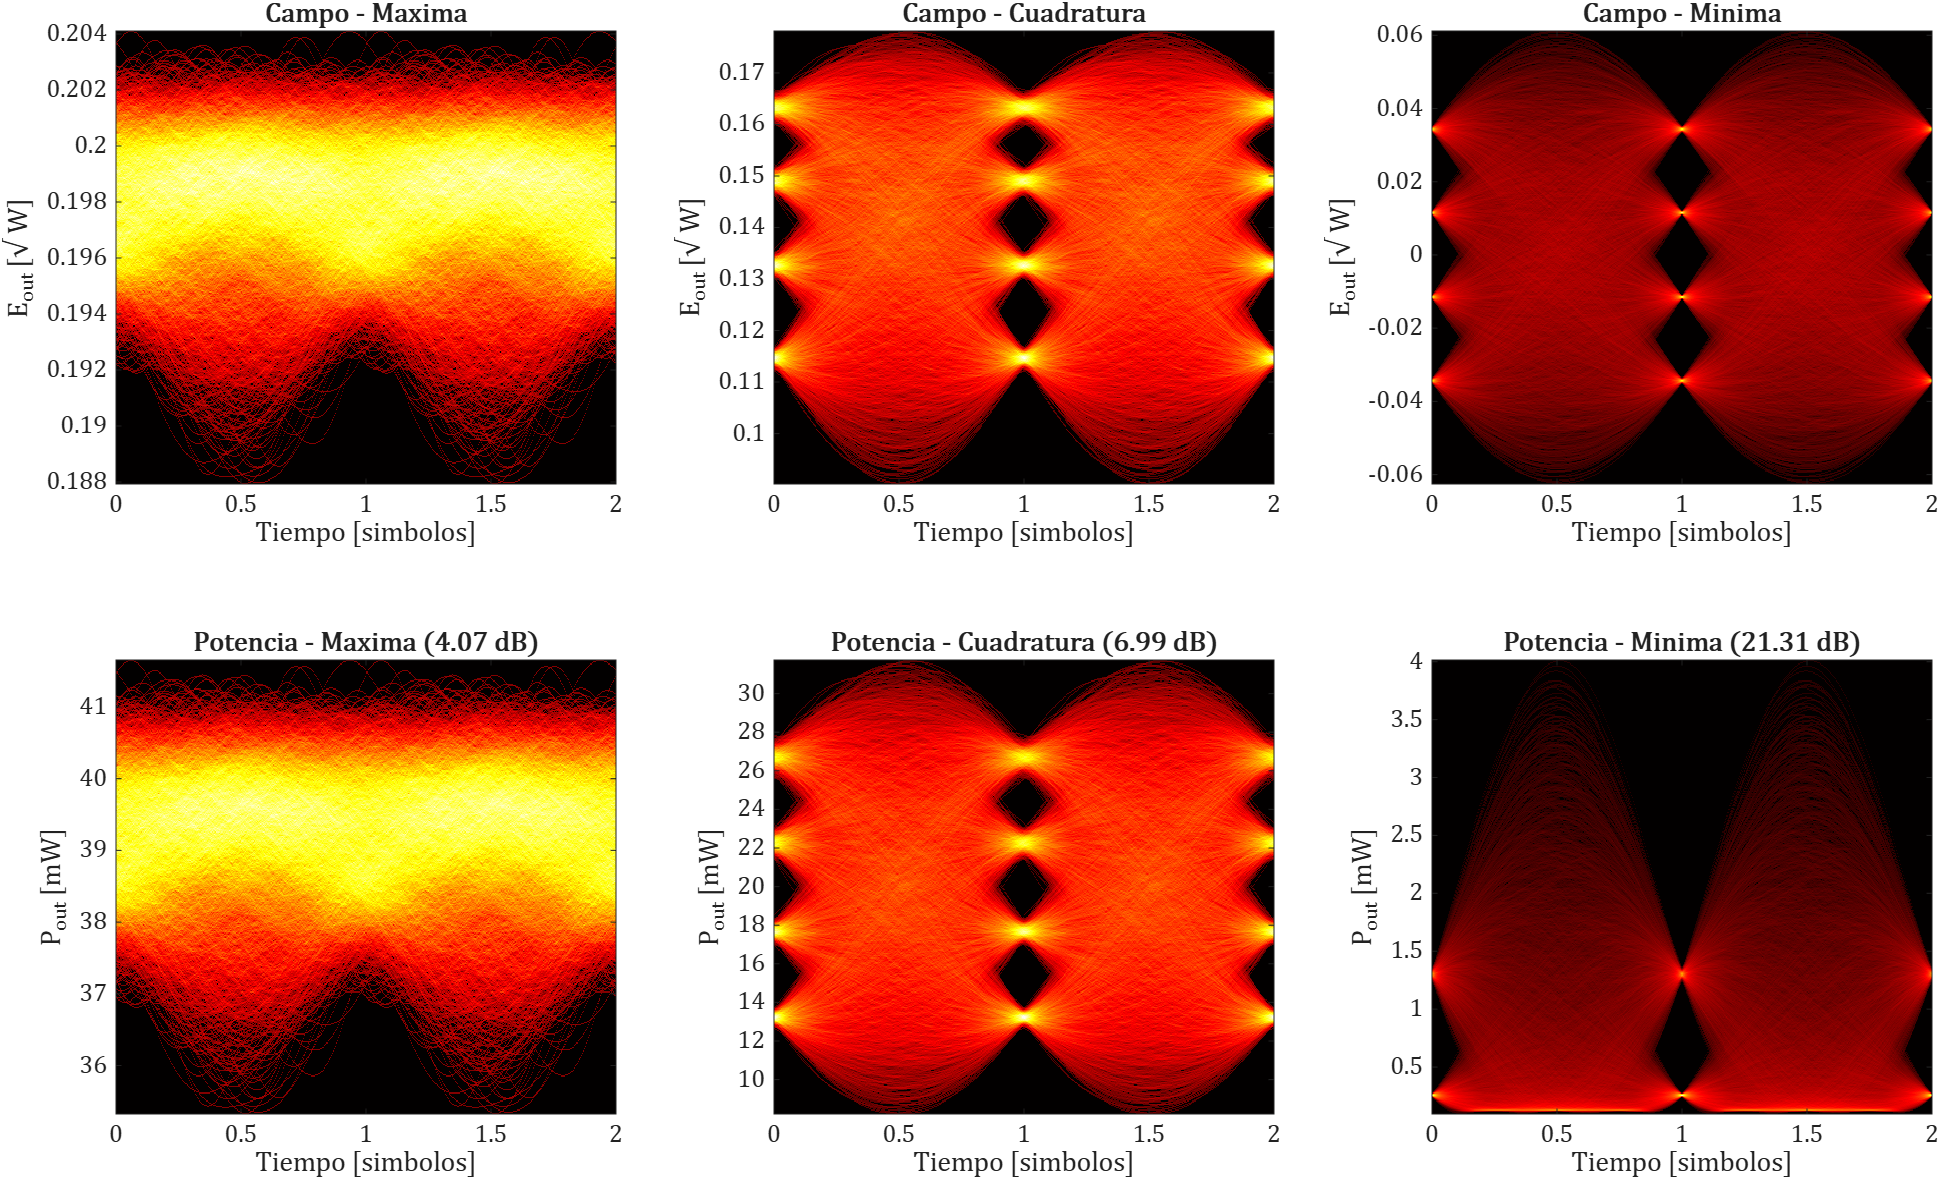
\includegraphics[width=\textwidth]{figuras/ej5_ojos.png}
\caption{Diagramas de ojo a la salida del MZM: campo eléctrico (arriba) y
potencia óptica (abajo) en máxima, cuadratura y mínima.}
\label{fig:ej5_ojos}
\end{figure}

Para interpretar los ojos, la Tabla~\ref{tab:ej5_niveles} muestra la
potencia de salida en el instante de muestreo para cada uno de los cuatro
símbolos.

\begin{table}[H]
\centering
\small
\begin{tabular}{lcccc}
\toprule
& \multicolumn{4}{c}{Potencia en el instante de muestreo [mW]} \\
\cmidrule(lr){2-5}
Punto & $-0.551$ V & $-0.184$ V & $+0.184$ V & $+0.551$ V \\
\midrule
Máxima     & $38.62$ & $39.70$ & $39.67$ & $38.61$ \\
Cuadratura & $26.69$ & $22.27$ & $17.68$ & $13.23$ \\
Mínima     & $1.303$ & $0.258$ & $0.258$ & $1.302$ \\
\bottomrule
\end{tabular}
\caption{Potencia óptica de salida para cada símbolo PAM4.}
\label{tab:ej5_niveles}
\end{table}

\paragraph{Máxima.}
Es el punto de menor pérdida: $4.07$~dB, apenas $0.07$~dB por encima de la
pérdida de inserción, porque la señal se mantiene cerca del máximo de la
curva de transferencia. Sin embargo el ojo está cerrado. Alrededor del
máximo la potencia es una función par de la tensión, de modo que los
símbolos $+v$ y $-v$ producen la misma potencia y los cuatro niveles
colapsan en dos. Además, por la pendiente casi nula, esos dos niveles
quedan separados por sólo $1.1$~mW (un $3$~\% de la potencia media), del
orden de las fluctuaciones del RIN del láser.

\paragraph{Cuadratura.}
La pérdida es de $6.99$~dB: a los $4$~dB de inserción se suman $3$~dB
porque en este punto se transmite, en promedio, la mitad de la potencia.
Es el único punto en el que los cuatro niveles de potencia son distintos y
prácticamente equiespaciados (separaciones de $4.4$, $4.6$ y $4.5$~mW), lo
que se traduce en un ojo abierto con cuatro niveles bien definidos. El
orden de los niveles queda invertido respecto de la señal eléctrica porque
la pendiente de la curva es negativa en $V_\pi/2$.

\paragraph{Mínima.}
La pérdida asciende a $21.31$~dB, ya que el modulador trabaja en el valle
de la curva de transferencia y casi toda la potencia se extingue. Igual que
en máxima, la potencia es una función par de la tensión y los cuatro
símbolos colapsan en dos niveles ($1.30$ y $0.26$~mW). El diagrama de ojo
del campo, en cambio, conserva los cuatro niveles, bipolares y
equiespaciados: alrededor del cruce por cero el campo es proporcional a la
señal. La información está en el campo y no en la potencia.

En este punto también se aprecia el ER finito: de los $0.258$~mW de los
símbolos interiores, $0.126$~mW corresponden al piso de potencia que deja
la extinción incompleta (Ejercicio~4). Con un modulador de $ER = \infty$ la
pérdida sería de $22.1$~dB.

\paragraph{Conclusión.}
La pérdida de potencia y la calidad del ojo no van de la mano. Máxima es el
punto más eficiente en potencia pero no transmite la señal; mínima es el
más lineal en campo pero el de mayor pérdida, y su información no es
recuperable midiendo potencia. Para modulación de intensidad el punto de
operación es cuadratura, que cuesta $3$~dB adicionales de pérdida a cambio
de una respuesta lineal en potencia.

%==========================================================================
\subsection*{Ejercicio 9: Implementación del modelo de un MZM-IQ ideal}
%==========================================================================
% Figuras y datos: tests/test_MZM_IQ_ex9.m

\subsubsection*{Configuración}

El modulador IQ se implementó con dos MZM en paralelo, uno por rama, cada
uno con el modelo de los ejercicios anteriores. El campo del láser pasa por
la pérdida de inserción del IQ, se divide en un acoplador con $K = 0.5$, se
modula en cada rama, la rama Q recibe el desfasaje $\phi$ y ambas se
recombinan en un segundo acoplador con $K = 0.5$. Se usaron los parámetros
de la consigna: $V_\pi = 5$~V, $ER = \infty$, $IL_{IQ} = 3$~dB e
$IL_{MZM} = 4$~dB, con el láser de $20$~dBm.

A cada rama se le inyectó una señal PAM4 independiente con las mismas
características que en el Ejercicio~5 ($240$~Gbaud, coseno realzado de
roll-off $0.2$, $2$~V$_{pp}$ sobre la forma de onda, $f_s = 960$~GHz). Los
puntos de polarización son los obtenidos en el Ejercicio~8: ambos MZM en
mínima, $V_{Bias,i} = V_{Bias,q} = V_\pi = 5$~V, y
$V_{Bias,\phi} = V_\pi/2 = 2.5$~V para que $\phi = \pi/2$.

\subsubsection*{Verificación de los apartados a) y b)}

Bajo estas condiciones el campo de salida debe ser
%
\begin{equation}
E_{out}(t) = \frac{E_{in}(t)}{2\sqrt{IL_{IQ}\,IL_{MZM}}}
\left[\sin\!\left(\frac{\pi x_i(t)}{2V_\pi}\right)
+ j\,\sin\!\left(\frac{\pi x_q(t)}{2V_\pi}\right)\right],
\label{eq:ej9_eout}
\end{equation}
%
con las pérdidas en escala lineal de potencia. El signo global de la
expresión depende de la convención de fase de los acopladores y no afecta
ningún resultado. La Figura~\ref{fig:ej9_teo} compara las partes real e
imaginaria del campo simulado con la ecuación~(\ref{eq:ej9_eout}): las
curvas se superponen y la máxima diferencia en toda la simulación es de
$2.3\times10^{-17}~\sqrt{\text{W}}$. La
parte real corresponde a la rama I y la imaginaria a la rama Q, lo que
confirma el desfasaje de $\pi/2$ entre ramas.

\begin{figure}[H]
\centering
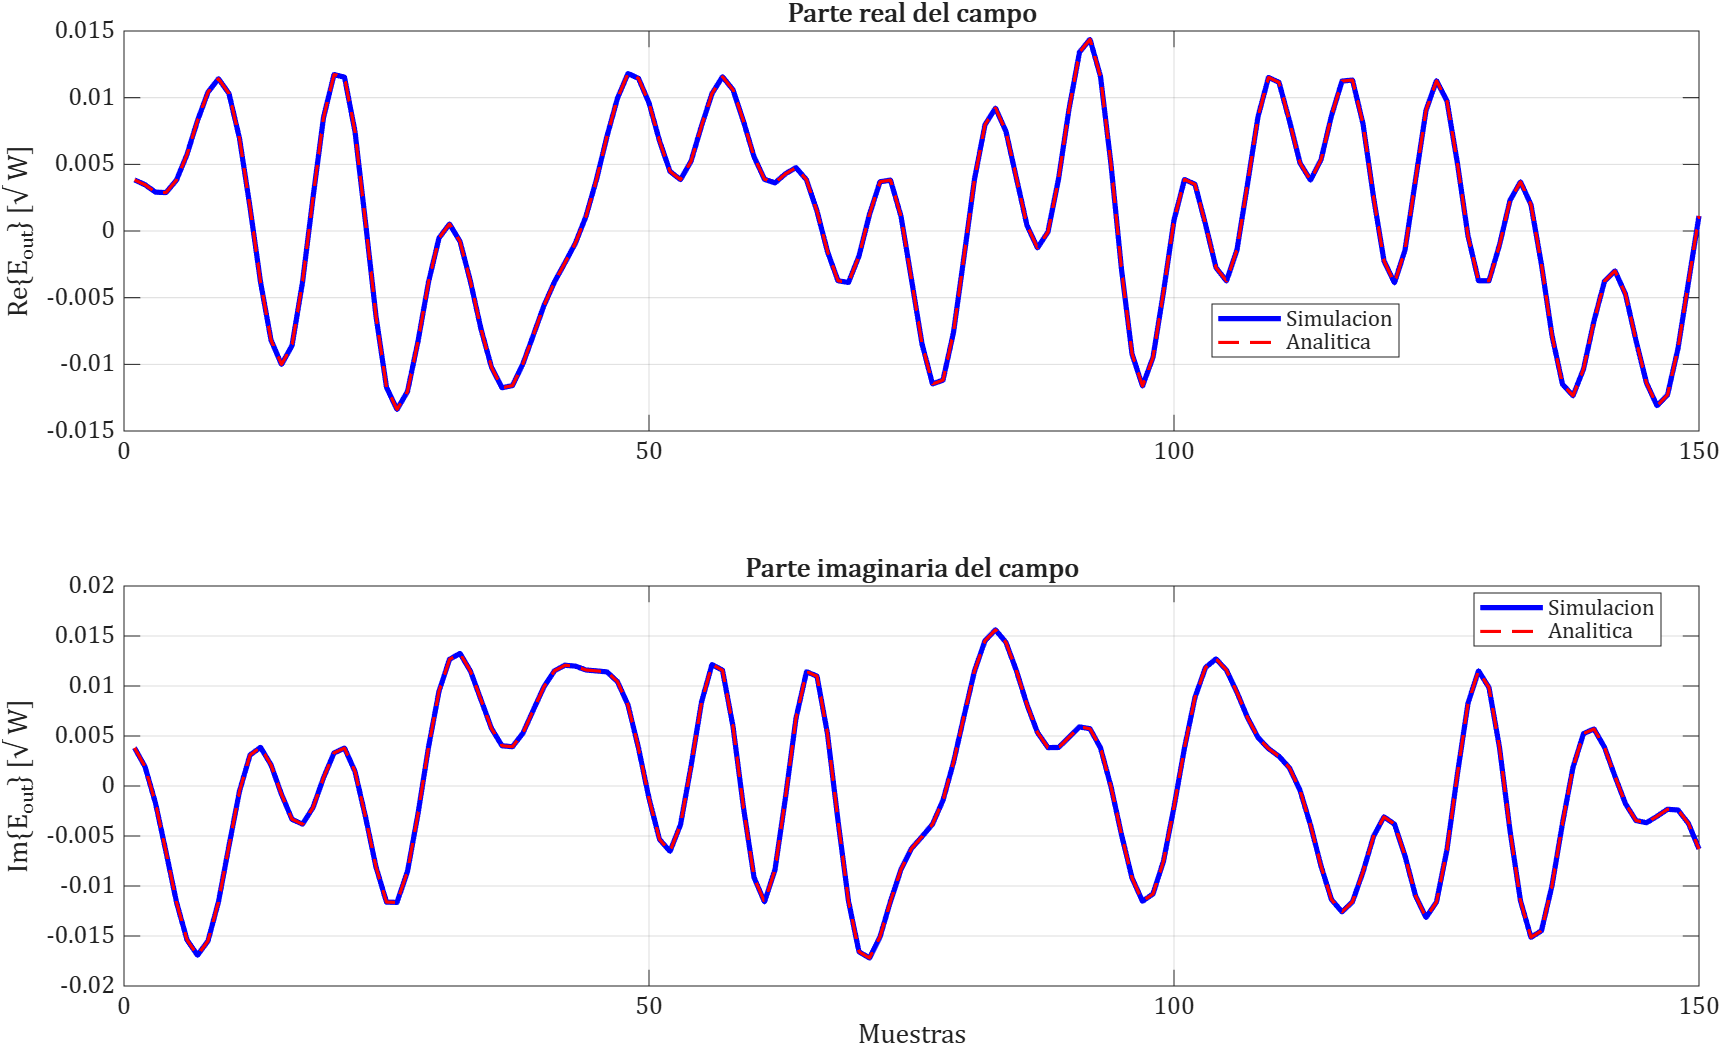
\includegraphics[width=0.9\textwidth]{figuras/ej9_campo_teo.png}
\caption{Partes real e imaginaria del campo de salida del MZM-IQ:
simulación y expresión analítica.}
\label{fig:ej9_teo}
\end{figure}

\subsubsection*{Verificación de los apartados c) y d)}

La potencia media de salida que predice el Ejercicio~8 es
%
\begin{equation}
\langle P_{out}\rangle = \frac{P_{in}}{4\,IL_{IQ}\,IL_{MZM}}
\left\langle \sin^2\!\left(\frac{\pi x_i}{2V_\pi}\right)
+ \sin^2\!\left(\frac{\pi x_q}{2V_\pi}\right)\right\rangle,
\end{equation}
%
y la pérdida por modulación es
$L_{mod} = 10\log_{10}(P_{in}/\langle P_{out}\rangle)$. La
Tabla~\ref{tab:ej9_potencia} compara ambos valores con los obtenidos de la
simulación.

\begin{table}[H]
\centering
\small
\begin{tabular}{lcc}
\toprule
& Analítico & Simulado \\
\midrule
$\langle P_{out}\rangle$ [mW] & $0.140186$ & $0.140180$ \\
$L_{mod}$ [dB]                & $28.533$   & $28.533$ \\
\bottomrule
\end{tabular}
\caption{Potencia media de salida y pérdida por modulación del MZM-IQ
($P_{in} = 100$~mW).}
\label{tab:ej9_potencia}
\end{table}

Los valores analíticos y simulados coinciden: la diferencia relativa en
la potencia es de $4\times10^{-5}$ y se debe al RIN del láser, y la
pérdida por modulación es la misma con tres decimales.

\subsubsection*{Diagramas de ojo y constelación}

La Figura~\ref{fig:ej9_ojos} muestra los diagramas de ojo de las
componentes I y Q del campo y de la potencia óptica. Para graficarlos se
compensó la fase del láser, como lo haría un receptor coherente con
recuperación de portadora ideal; de lo contrario el ruido de fase mezcla
las dos componentes.

\begin{figure}[H]
\centering
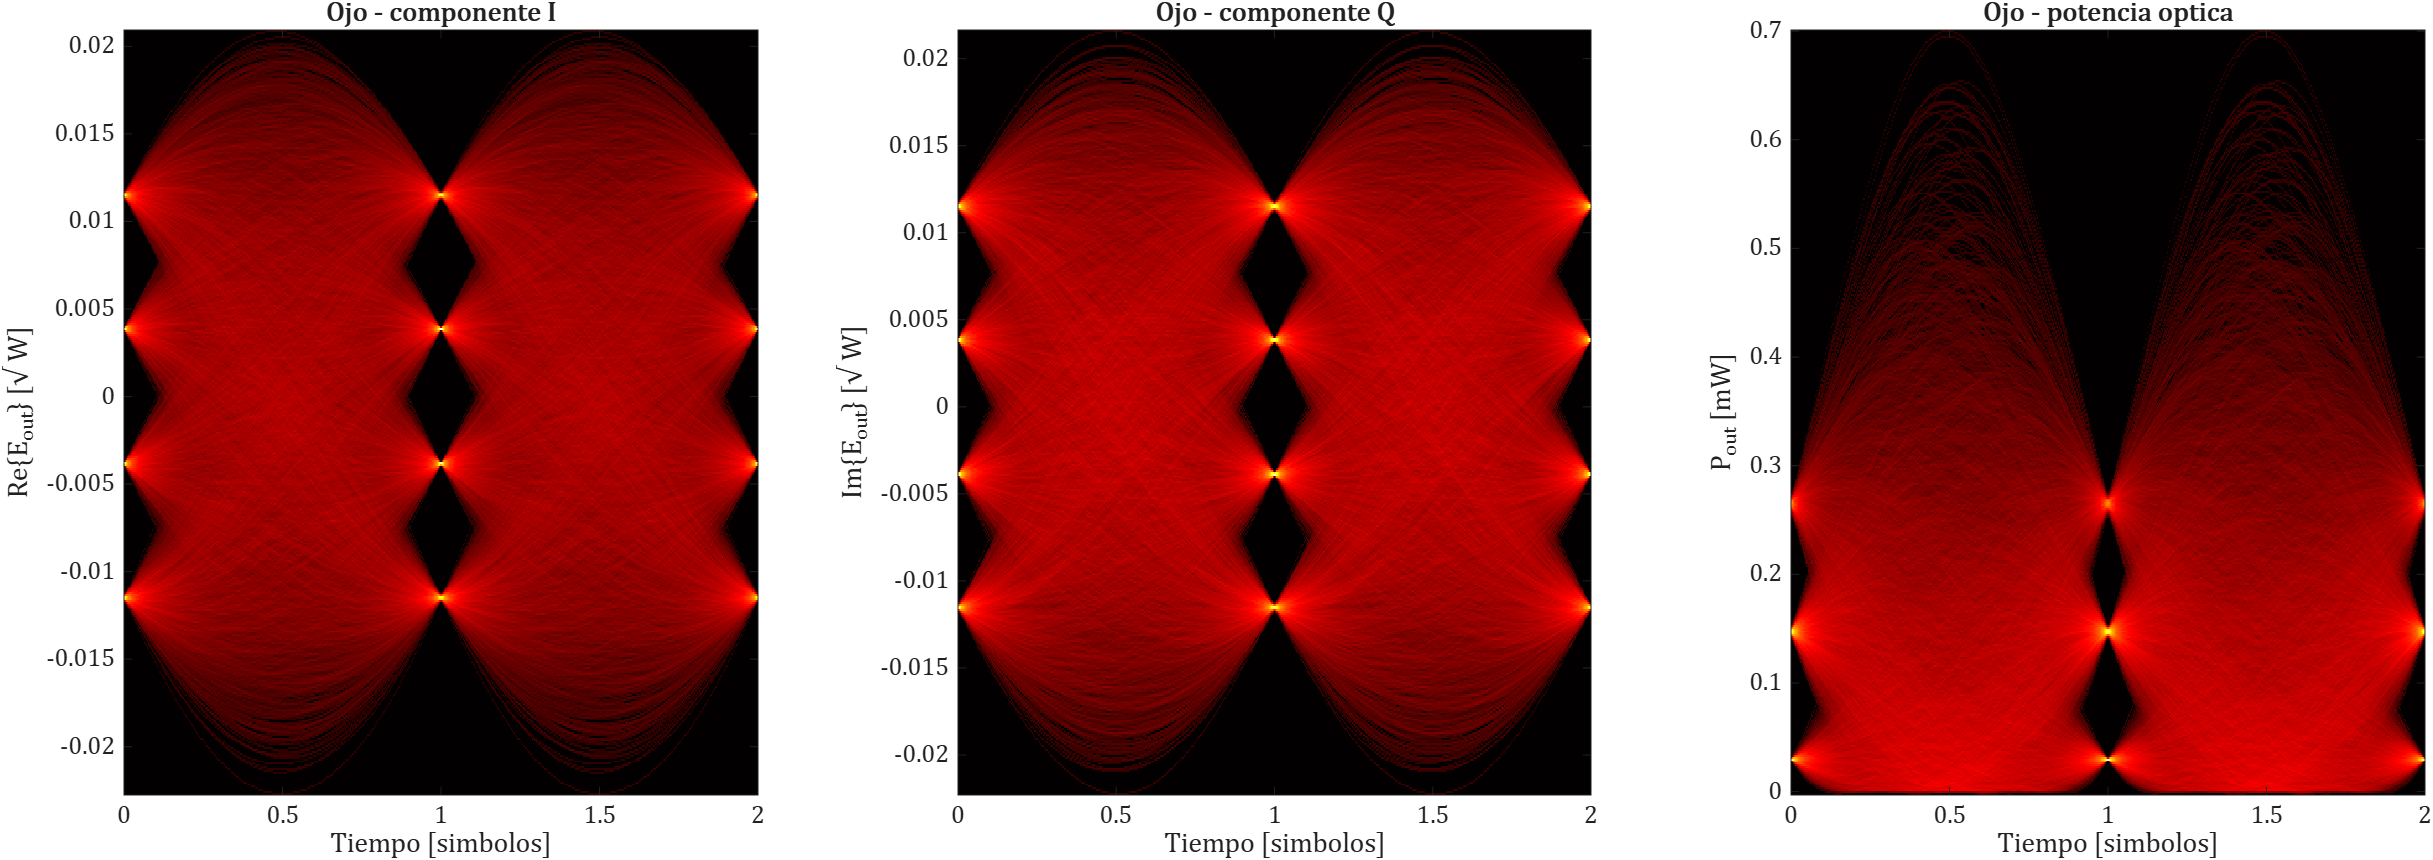
\includegraphics[width=\textwidth]{figuras/ej9_ojos.png}
\caption{Diagramas de ojo a la salida del MZM-IQ: componente I, componente
Q y potencia óptica.}
\label{fig:ej9_ojos}
\end{figure}

Las componentes I y Q presentan cuatro niveles bipolares y equiespaciados
cada una, igual que el campo del MZM polarizado en mínima del Ejercicio~5.
El ojo de potencia, en cambio, tiene tres niveles ($0.03$, $0.15$ y
$0.27$~mW): la potencia es $|E_I|^2 + |E_Q|^2$ y los dieciséis símbolos
sólo toman tres valores de módulo, según cuántas de sus dos componentes
estén en el nivel externo.

\begin{figure}[H]
\centering
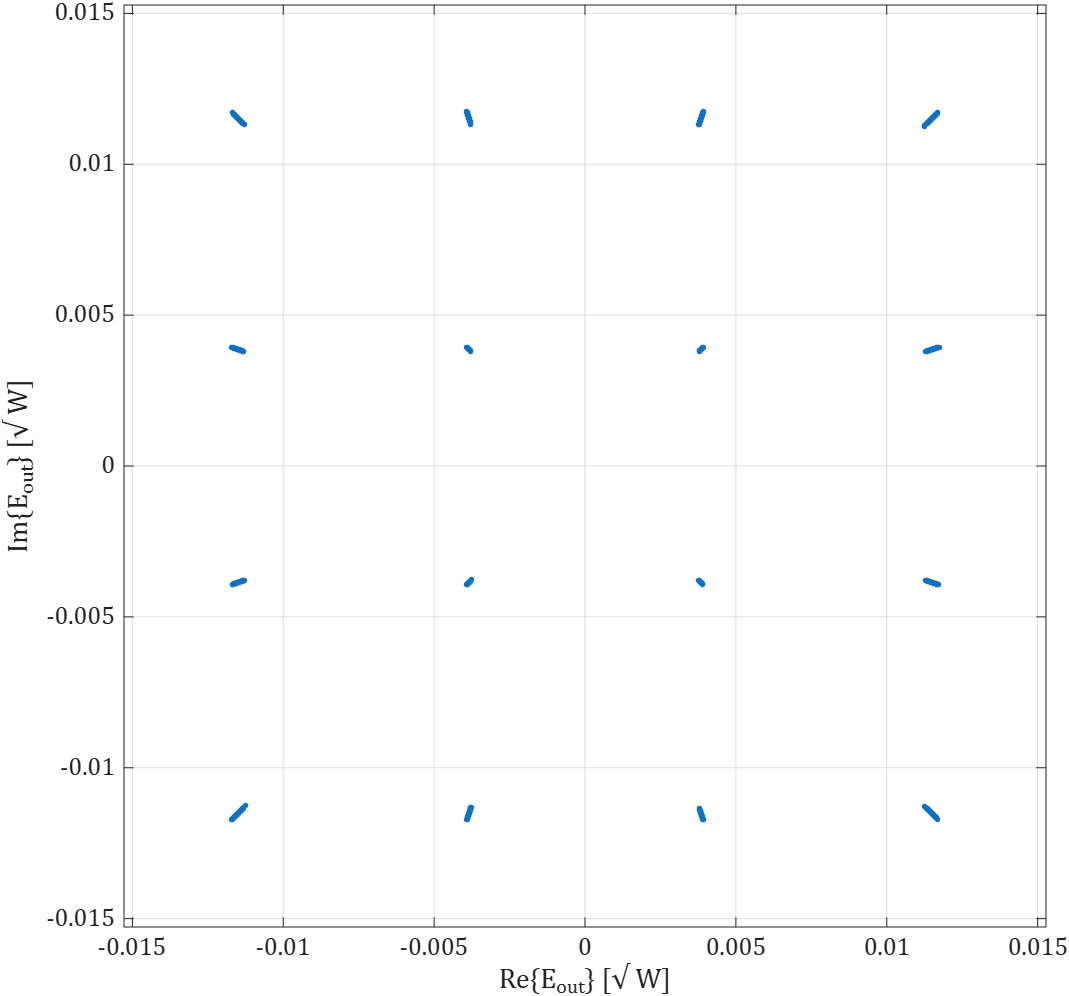
\includegraphics[width=0.55\textwidth]{figuras/ej9_constelacion.png}
\caption{Constelación a la salida del MZM-IQ en los instantes de
muestreo.}
\label{fig:ej9_const}
\end{figure}

En los instantes de muestreo el campo forma una constelación 16-QAM
(Figura~\ref{fig:ej9_const}), como corresponde a dos señales PAM4
independientes en cuadratura. Cada punto se estira en dirección radial por
el RIN, que escala la amplitud del campo sin cambiar su fase; por eso los
segmentos son más largos en los puntos exteriores. Sin el ruido del
láser, cada componente coincide con el nivel ideal $\sin(\pi x/2V_\pi)$ de
su símbolo con un error de $2.2\times10^{-16}$: el pulso de coseno
realzado no introduce interferencia entre símbolos en el instante de
muestreo.

%==========================================================================
\subsection*{Ejercicio 10: Modulador DP-IQ}
%==========================================================================
% Figuras y datos: tests/test_MZM_DPIQ_ex10.m

\subsubsection*{Implementación}

El modulador de doble polarización se construyó a partir de dos
moduladores IQ como el del Ejercicio~9. El campo del láser pasa por la
pérdida de inserción $IL_{xy}$, se divide en partes iguales entre los dos
IQ, cada uno modula una de las polarizaciones con dos señales PAM4 propias,
y el PBC combina ambas salidas en modos de polarización ortogonales. La
salida es un vector de dimensión $2\times1$:
%
\begin{equation}
\mathbf{E}_{out}(t) =
\begin{bmatrix} E_{MZMx}(t) \\ E_{MZMy}(t) \end{bmatrix} =
\begin{bmatrix} E_{ix}(t) + jE_{qx}(t) \\ E_{iy}(t) + jE_{qy}(t) \end{bmatrix},
\end{equation}
%
que en la simulación se representa como una matriz de $2 \times N$
muestras. Cada IQ se polarizó igual que en el Ejercicio~9.

La consigna no especifica el valor de $IL_{xy}$; se adoptó
$IL_{xy} = 3$~dB, con $IL_{IQ} = 3$~dB e $IL_{MZM} = 4$~dB como en el
ejercicio anterior. Para aislar el comportamiento del modulador se
desactivaron el RIN y el ruido de fase del láser. Las cuatro señales PAM4
son independientes, por lo que el modulador transmite
$4 \times 2~\text{bits} \times 240~\text{Gbaud} = 1.92$~Tb/s.

\subsubsection*{Resultados}

El campo simulado en cada polarización coincide con la expresión del
Ejercicio~9 afectada por el divisor de entrada y por $IL_{xy}$, con una
diferencia máxima de $1.2\times10^{-17}~\sqrt{\text{W}}$. La
Figura~\ref{fig:ej10_ojos} muestra los diagramas de ojo de las cuatro
ramas: los cuatro son equivalentes, con cuatro niveles bien definidos, y
la Figura~\ref{fig:ej10_const} muestra la constelación 16-QAM de cada
polarización.

\begin{figure}[H]
\centering
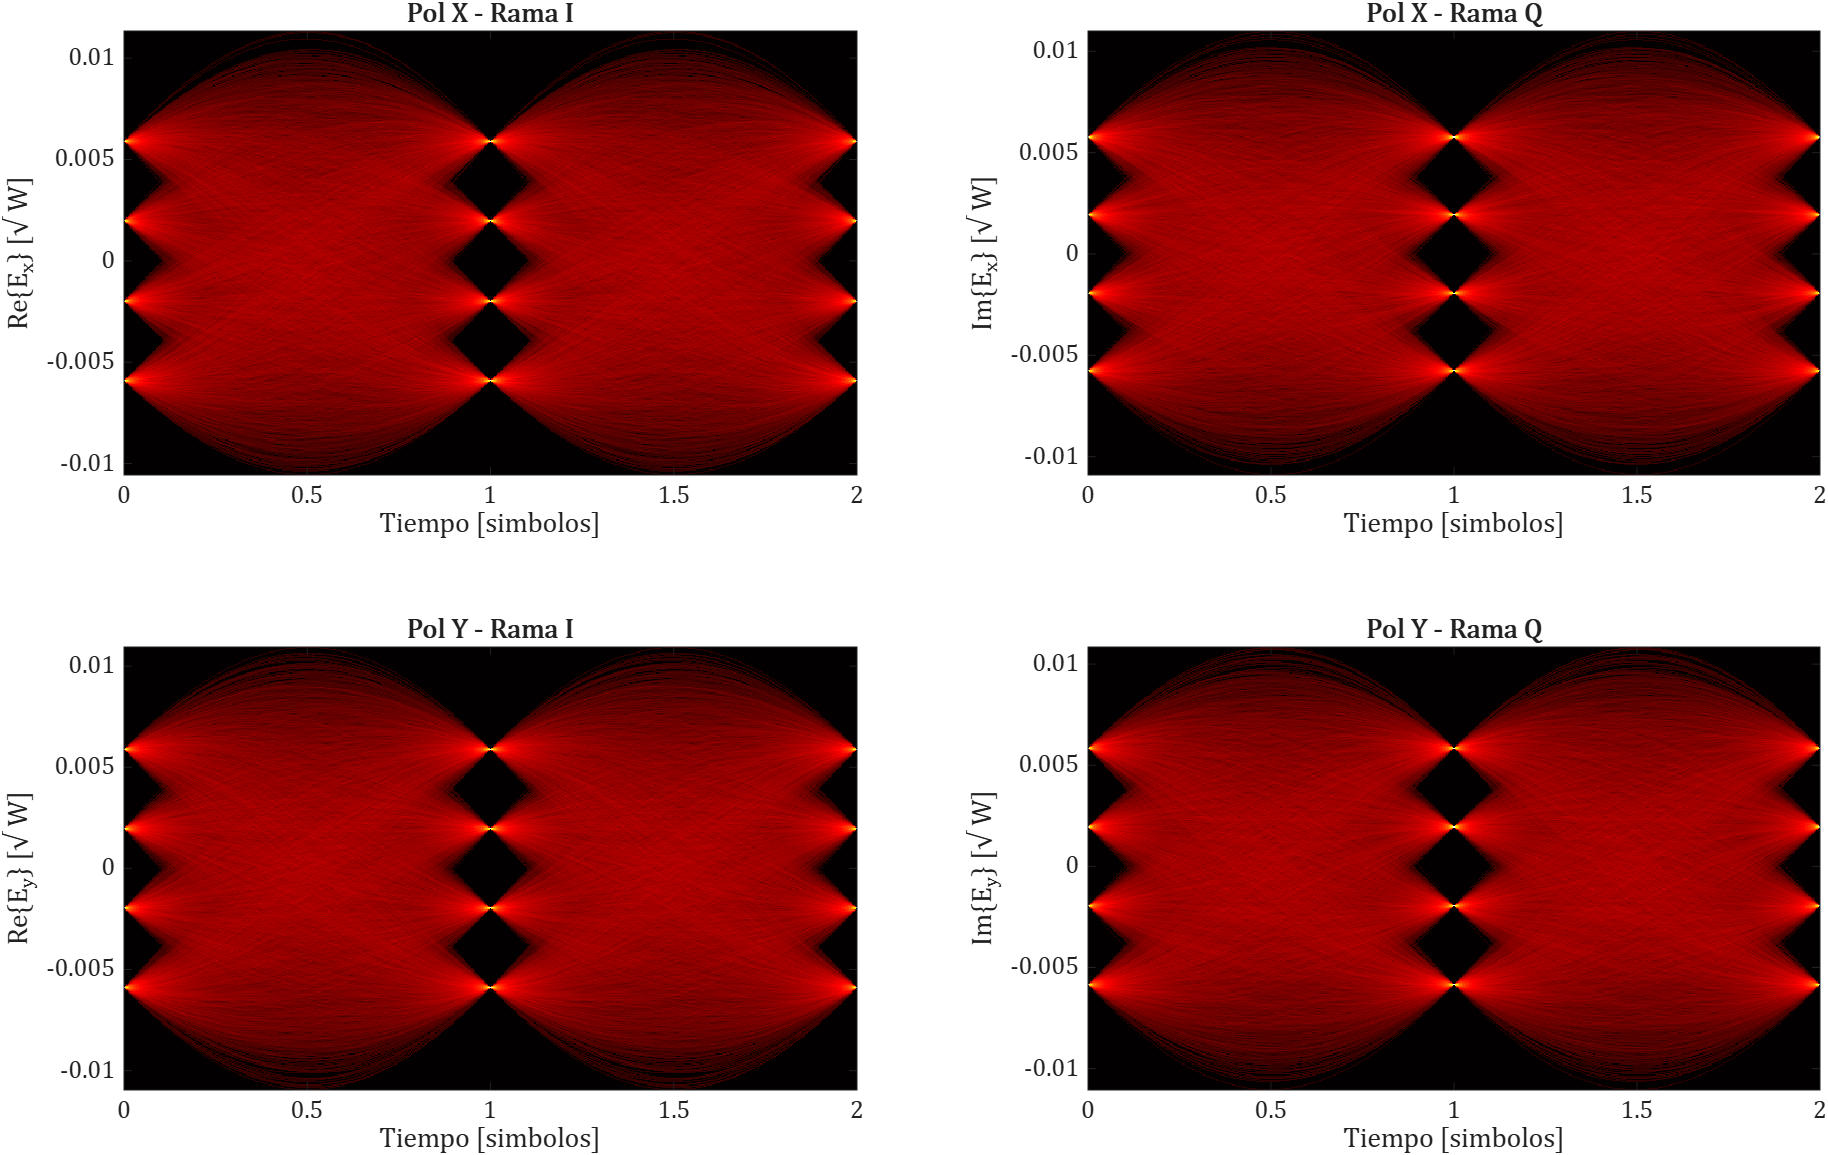
\includegraphics[width=\textwidth]{figuras/ej10_ojos.png}
\caption{Diagramas de ojo de las ramas I y Q de las polarizaciones $x$ e
$y$ del modulador DP-IQ.}
\label{fig:ej10_ojos}
\end{figure}

\begin{figure}[H]
\centering
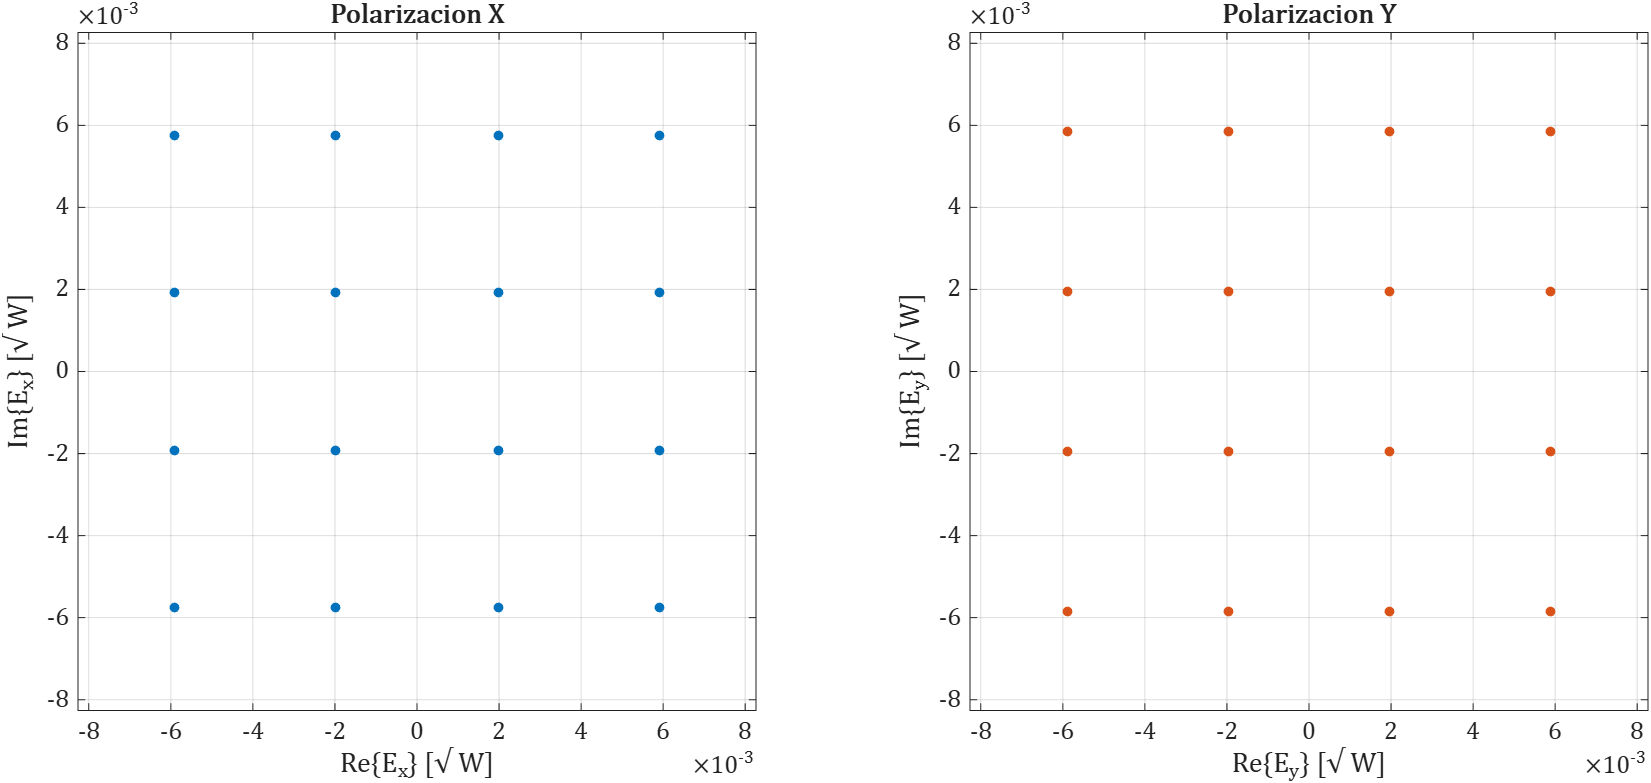
\includegraphics[width=0.9\textwidth]{figuras/ej10_constelacion.png}
\caption{Constelación 16-QAM en cada polarización del modulador DP-IQ.}
\label{fig:ej10_const}
\end{figure}

\begin{table}[H]
\centering
\small
\begin{tabular}{lcc}
\toprule
& $\langle P_{out}\rangle$ [mW] & Pérdida [dB] \\
\midrule
Polarización $x$ & $0.0360$ & $34.44$ \\
Polarización $y$ & $0.0366$ & $34.37$ \\
Total            & $0.0725$ & $31.40$ \\
\bottomrule
\end{tabular}
\caption{Potencia media de salida por polarización y total
($P_{in} = 100$~mW).}
\label{tab:ej10_potencia}
\end{table}

La Tabla~\ref{tab:ej10_potencia} resume las potencias de salida. Las dos
polarizaciones transportan la misma potencia (la diferencia de
$0.07$~dB es estadística, por usar secuencias distintas), y la pérdida
total de $31.4$~dB se compone de los $3$~dB de $IL_{xy}$ más los
$28.4$~dB de un modulador IQ. El reparto entre polarizaciones no aparece en
la pérdida total: cada polarización recibe la mitad de la potencia, pero
el PBC combina modos ortogonales y sus potencias se suman sin pérdida. Por
eso la pérdida medida sobre una sola polarización es $3$~dB mayor.
